\thispagestyle{thachthuctoanhocnone}
\pagestyle{thachthuctoanhoc}
\everymath{\color{thachthuctoanhoc}}
\graphicspath{{../thachthuctoanhoc/pic/}}
\begingroup
\AddToShipoutPicture*{\put(0,616){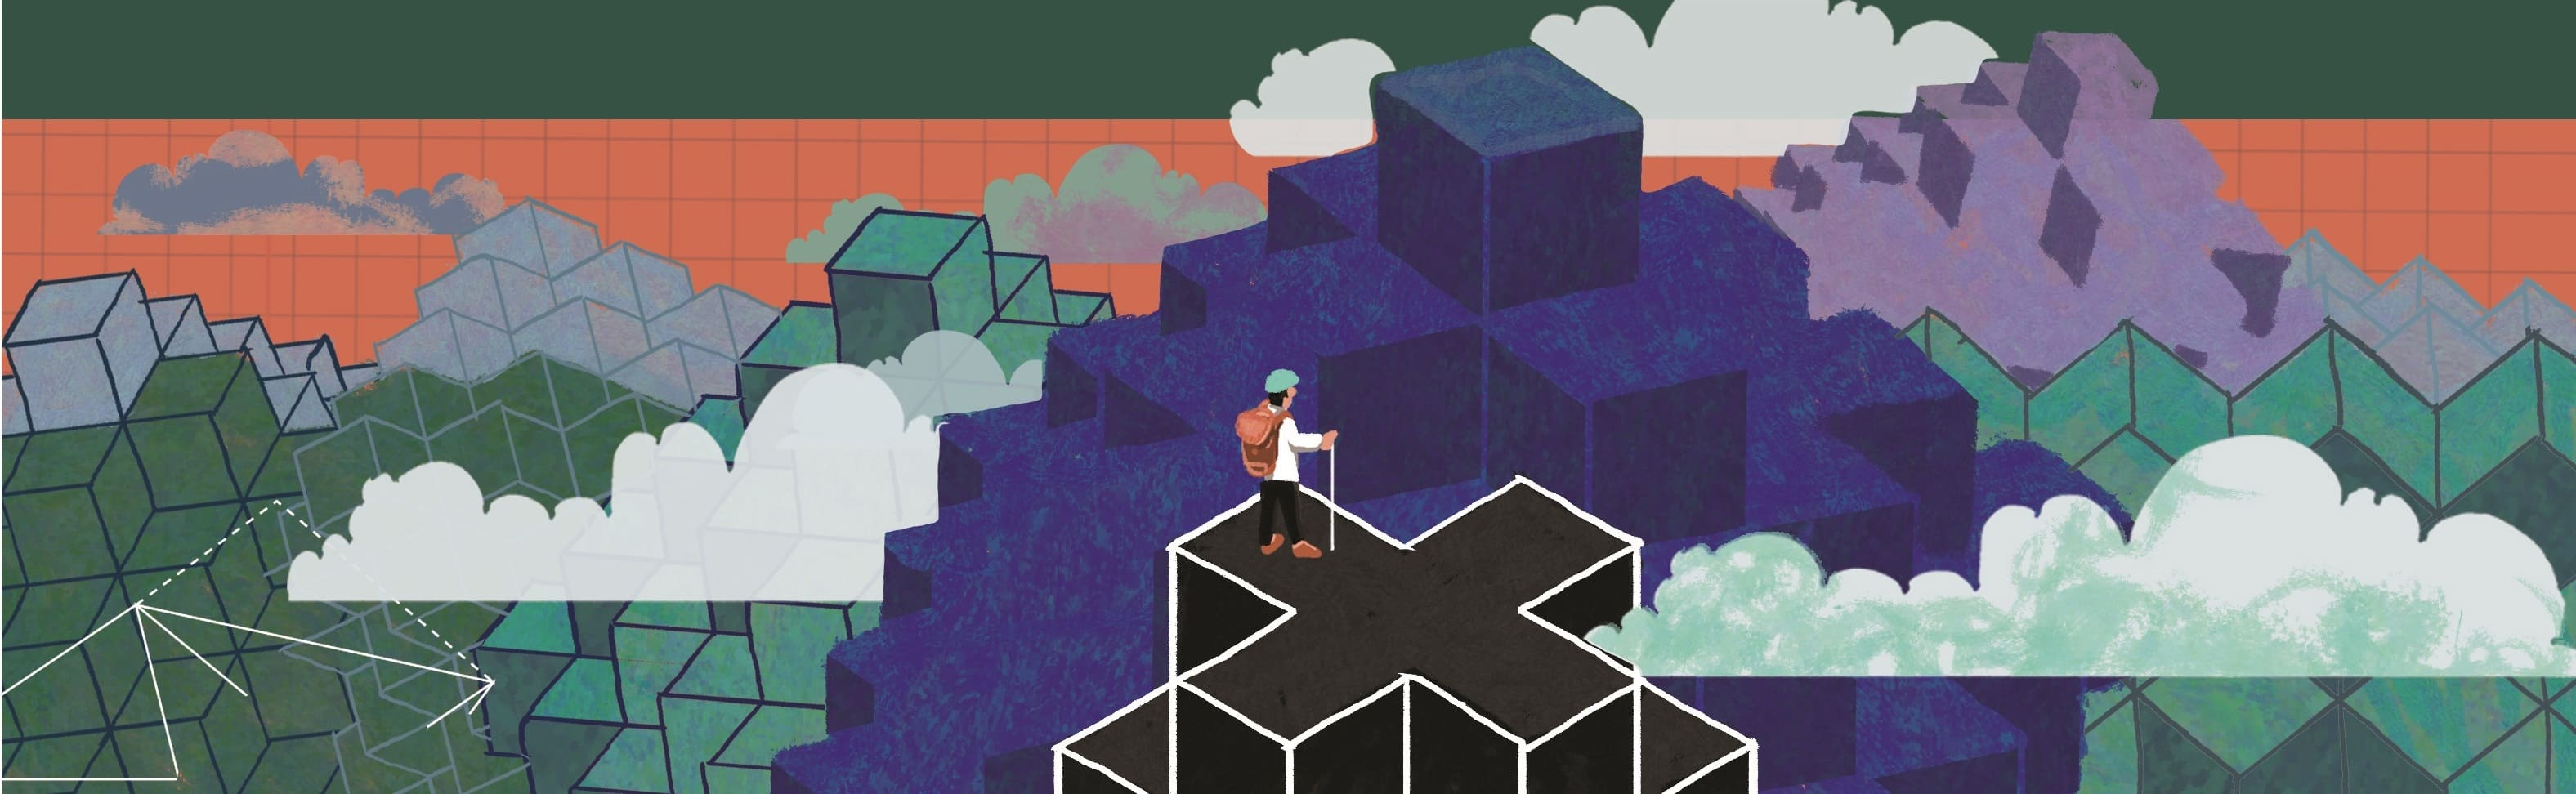
\includegraphics[width=19.3cm]{../thachthuctoanhoc/bannerthachthuc}}}
\centering
\vspace*{4cm}
\endgroup
\vspace*{-8pt}
\begin{tBox}
	\begin{itemize}[leftmargin = 13pt, itemsep = 1.0pt] 
		\item Mỗi bài toán đề xuất (kèm theo lời giải) cần được nêu rõ là bài sáng tác hay bài sưu tầm.
		%		\item Mỗi bài toán đề xuất (kèm theo lời giải) cần được nêu rõ là bài sáng tác hay bài sưu tầm (nếu là bài sưu tầm, cần ghi rõ nguồn).
		\item Bài giải cho mỗi bài toán cần được trình bày trong một file riêng hoặc
		một tờ giấy riêng.
		\item  Người đề xuất bài toán hoặc gửi bài giải cho các bài toán trong mục ``Thách thức kỳ này" cần ghi rõ họ, đệm, tên và nơi làm việc/học tập, số điện thoại liên hệ. Nếu là học sinh (hoặc sinh viên) cần ghi rõ là học sinh lớp mấy (hoặc sinh viên năm thứ mấy).
		\item Các bài toán trong mục Thách thức kỳ này hướng tới các độc giả là học sinh phổ thông; được phân chia thành các mức độ $B$, $A$, và được sắp xếp theo độ khó tăng dần, theo đánh giá chủ quan của Ban biên tập. Các bài toán mức độ $B$ không đòi hỏi các kiến thức vượt quá chương trình môn Toán cấp THCS; các bài toán mức độ $A$ không đòi hỏi các kiến thức vượt quá chương trình môn Toán cấp THPT.
		\item Cách thức gửi bài toán đề xuất hoặc lời giải: gửi file thu được bằng cách scan, ảnh chụp (rõ nét) của bản viết tay, hoặc được soạn thảo bằng các phần mềm Latex, Word tới \url{bbt@pi.edu.vn} hoặc gửi qua đường bưu điện tới Tòa soạn (xem địa chỉ tại bìa $2$).
		\item Hạn gửi lời giải cho các bài toán P$781$--P$790$: trước ngày $15/3/2024$.
	\end{itemize}
\end{tBox}
\begin{center}
	\vspace*{-5pt}
	\textbf{\color{thachthuctoanhoc}\color{thachthuctoanhoc}\color{thachthuctoanhoc}\color{thachthuctoanhoc}\color{thachthuctoanhoc}THÁCH THỨC KỲ NÀY}
	\vspace*{-5pt}
\end{center}
\begin{multicols}{2}
	\setlength{\abovedisplayskip}{4pt}
	\setlength{\belowdisplayskip}{4pt}
	{\color{thachthuctoanhoc}{\usefont{T5}{qag}{b}{n} P781.}}
	(Mức $B$) Chuẩn bị quà tặng cho nhân viên dịp Tết Giáp Thìn hai doanh nghiệp ${A}$ và ${B}$ đến một cơ sở sản xuất rượu vang để mua hàng. Cơ sở này có $6$ thùng rượu vang: Thùng $1$ chứa $310$ lít, thùng $2$ chứa $200$ lít, thùng $3$ chứa $190$ lít, thùng $4$ chứa $180$ lít, thùng $5$ chứa $160$ lít, thùng $6$ chứa $150$ lít. Doanh nghiệp $A$ mua $2$ thùng, doanh nghiệp $B$ mua $3$ thùng và số lượng mua gấp đôi số lượng mua của doanh nghiệp ${A}$. Theo bạn cơ sở sản xuất rượu vang còn lại thùng nào chưa bán? Mỗi doanh nghiệp đã mua bao nhiêu lít rượu vang?
	\begin{flushright}
		\textit{Nguyễn Thanh Giang, Hưng Yên}
	\end{flushright}
	{\color{thachthuctoanhoc}{\usefont{T5}{qag}{b}{n} P782.}}
	(Mức $B$) Cho tam giác $ABC$ cân tại $B$ có $\angle{ABC}=40^\circ.$ Gọi $M$ là điểm nằm trong tam giác sao cho ${BM}={AC}$ và $\angle{ABM}=10^{\circ}$. Tìm số đo của góc $\angle{AMC}.$
	\begin{center}
		\definecolor{qqwuqq}{rgb}{0.,0.39215686274509803,0.}
		\definecolor{ududff}{rgb}{0.30196078431372547,0.30196078431372547,1.}
		\definecolor{uuuuuu}{rgb}{0.26666666666666666,0.26666666666666666,0.26666666666666666}
		\begin{tikzpicture}[thachthuctoanhoc,scale=1.3]
			\draw [shift={(1.44,3.96)},color=qqwuqq,fill=qqwuqq,fill opacity=0.10000000149011612] (0,0) -- (-109.98310652189998:0.6) arc (-109.98310652189998:-69.98310652189998:0.6) -- cycle;
			\draw [shift={(1.44,3.96)},color=qqwuqq,fill=qqwuqq,fill opacity=0.10000000149011612] (0,0) -- (-109.98310652189998:0.9) arc (-109.98310652189998:-99.98310652189998:0.9) -- cycle;
			\draw  (0.,0.)-- (1.44,3.96);
			\draw [shift={(1.44,3.96)},color=qqwuqq] (-109.98310652189998:0.6) arc (-109.98310652189998:-69.98310652189998:0.6);
			\draw [shift={(1.44,3.96)},color=qqwuqq] (-109.98310652189998:0.47) arc (-109.98310652189998:-69.98310652189998:0.47);
			\draw  (1.44,3.96)-- (2.8823349362673674,8.498473002305218E-4);
			\draw  (2.8823349362673674,8.498473002305218E-4)-- (0.,0.);
			\draw  (1.4912028475775996,-0.11956032879327154) -- (1.4911320843430351,0.12043966077457186);
			\draw  (1.3912028519243316,-0.11958981347434133) -- (1.3911320886897673,0.12041017609350206);
			\draw  (1.44,3.96)-- (0.9407295282418738,1.1236063397281366);
			\draw  (1.3172157234336206,2.5702431790316433) -- (1.080849585077632,2.6118490516781545);
			\draw  (1.299879943164241,2.471757288049982) -- (1.0635138048082526,2.513363160696493);
			\draw  (0.9407295282418738,1.1236063397281366)-- (0.,0.);
			\draw  (0.9407295282418738,1.1236063397281366)-- (2.8823349362673674,8.498473002305218E-4);
			\draw [fill=white] (0.,0.) circle (1.5pt);
			\draw (-0.36,-0.19) node {$A$};
			\draw [fill=white] (1.44,3.96) circle (1.5pt);
			\draw (1.58,4.33) node {$B$};
			\draw [fill=white] (2.8823349362673674,8.498473002305218E-4) circle (1.5pt);
			\draw (3.2,-0.21) node {$C$};
			\draw [fill=white] (0.9407295282418738,1.1236063397281366) circle (1.5pt);
			\draw (1.28,1.33) node {$M$};
			\draw (1.56,3) node {\scriptsize$40^\circ$};
			\draw (1.2,2.8) node {\scriptsize$10^\circ$};
		\end{tikzpicture}
	\end{center}
	\begin{flushright}
		\textit{Đỗ Thanh Sơn, Hà Nội}
	\end{flushright}
	{\color{thachthuctoanhoc}{\usefont{T5}{qag}{b}{n} P783.}}
	(Mức $B$) Cho các số hữu tỷ $a,b,c$ thoả mãn $(a+bc)(b+ac)(a+b)\ne0$  và
	\begin{align*}
		\dfrac1{a+bc}+\dfrac1{b+ac}=\dfrac2{a+b}.
	\end{align*}
	Chứng minh rằng, $c^2-1$ là bình phương của một số hữu tỷ.
	\begin{flushright}
		\textit{Phạm Nhật Nguyệt, Hải Phòng}
	\end{flushright}
	{\color{thachthuctoanhoc}{\usefont{T5}{qag}{b}{n} P784.}}
	(Mức $B$) Tồn tại hay không $2024$ số nguyên tố lẻ đôi một phân biệt sao cho tổng của $11$ số bất kì trong $2024$ số đó đều là hợp số?
	\begin{flushright}
		\textit{ Đỗ Khải Phương, Hà Nội}
	\end{flushright}
	{\color{thachthuctoanhoc}{\usefont{T5}{qag}{b}{n} P785.}}
	(Mức $B$) Cho sáu số thực $a,b,c,x,y,z$ thỏa mãn $ax+by+cz=0$ và $a^2+b^2+1=c^2.$ 
	Chứng minh rằng $x^2+y^2-z^2\ge 0.$
	\begin{flushright}
		\textit{Phạm Công Tài, Hà Nội}
	\end{flushright}
	{\color{thachthuctoanhoc}{\usefont{T5}{qag}{b}{n} P786.}}
	(Mức $B$) Cho số nguyên dương $n\ge 4$ và $n$ điểm phân biệt trên mặt phẳng (không có $3$ điểm thẳng hàng). Bạn Trung vẽ $n+1$ đoạn thẳng có đầu mút là các điểm đã cho. Chứng minh rằng luôn tồn tại $2$ đoạn thẳng không có điểm chung.
	\begin{flushright}
		\textit{Lê Văn Kiệt, Vĩnh Phúc (sưu tầm)}
	\end{flushright}

	{\color{thachthuctoanhoc}{\usefont{T5}{qag}{b}{n} P787.}}
	(Mức $A$) Xét $a,b,c$ là các số thực thoả mãn 
	\begin{align*}
		a b^2+b c^2+c a^2=6 \sqrt{3}+a c^2+c b^2+b a^2.
	\end{align*}
	Tìm giá trị nhỏ nhất của biểu thức $P=a^2+b^2+c^2$.
	\begin{flushright}
		\textit{Trần Công Diêu, Tp. Hồ Chí Minh (st)}
	\end{flushright}
	{\color{thachthuctoanhoc}{\usefont{T5}{qag}{b}{n} P788.}}
	(Mức $A$) Cho tam giác nhọn $ABC$ có $AD, BE, CF$ là các đường cao. Gọi $X, Y$ là các điểm khác $D$, tương ứng thuộc các tia $DE, DF$ sao cho $DX = DY.$  Giả sử các đường tròn $(CDX), (BDY)$ cắt nhau tại điểm thứ hai $P$ (khác $D$). Chứng minh rằng khi $X, Y$ thay đổi thì $P$ luôn thuộc một đường thẳng cố định.
	
	Ở đây, $(XYZ)$ kí hiệu đường tròn ngoại tiếp tam giác $XYZ.$
	
	\begin{center}
		\definecolor{ffqqff}{rgb}{1,0,1}
		\definecolor{ffqqqq}{rgb}{1,0,0}
		\definecolor{qqzzff}{rgb}{0,0.6,1}
		\definecolor{qqqqff}{rgb}{0,0,1}
		\definecolor{qqqqffa}{rgb}{1,1,1}
		\begin{tikzpicture}[thachthuctoanhoc,scale=0.7]
			\draw[color=ffqqff] (-2.717157287525381,-2) -- (-2.717157287525381,-1.7171572875253809) -- (-3,-1.7171572875253809) -- (-3,-2) -- cycle; 
			\draw[color=ffqqff] (-1.086138249518438,1.261551458734635) -- (-0.9050667574334009,1.0442656682325906) -- (-0.6877809669313564,1.2253371603176277) -- (-0.8688524590163934,1.4426229508196722) -- cycle; 
			\draw[color=ffqqff] (-4.031671842700025,0.01055728090000839) -- (-3.9422291236000335,0.2788854381999832) -- (-4.210557280900008,0.3683281572999748) -- (-4.3,0.1) -- cycle; 
			\draw [color=qqzzff] (-3,4)-- (-5,-2);
			\draw [color=qqzzff] (-5,-2)-- (2,-2);
			\draw [color=qqzzff] (2,-2)-- (-3,4);
			\draw [color=ffqqqq] (-3,4)-- (-3,-2);
			\draw [color=ffqqqq] (-5,-2)-- (-0.8688524590163934,1.4426229508196722);
			\draw [color=ffqqqq] (-4.3,0.1)-- (2,-2);
			\draw  (-5.6505081967213115,2.2815901639344265)-- (-3,-2);
			\draw  (-3,-2)-- (-0.34949180327868845,2.2815901639344265);
			\draw  (-4,0.3421428571428573) circle (2.5466906296732055cm);
			\draw  (-0.5,-0.5864285714285713) circle (2.8719652128243944cm);
			\draw [fill=white] (-3,4) circle (1.5pt);
			\draw[color=qqqqff] (-2.98,4.44) node {$A$};
			\draw [fill=white] (-5,-2) circle (1.5pt);
			\draw[color=qqqqff] (-5.08,-2.28) node {$B$};
			\draw [fill=white] (2,-2) circle (1.5pt);
			\draw[color=qqqqff] (2.15,-2.28) node {$C$};
			\draw [fill=white] (-3,-2) circle (1.5pt);
			\draw[color=qqqqff] (-3.1,-2.28) node {$D$};
			\draw [fill=white] (-0.8688524590163934,1.4426229508196722) circle (1.5pt);
			\draw[color=qqqqff] (-0.54,1.6) node {$E$};
			\draw [fill=white] (-4.3,0.1) circle (1.5pt);
			\draw[color=qqqqff] (-4.62,0.1) node {$F$};
			\draw [fill=white] (-3,-0.3333333333333333) circle (1.5pt);
			%\draw[color=qqqqff] (-2.82,-0.66) node {$H$};
			\draw [fill=white] (-0.34949180327868845,2.2815901639344265) circle (1.5pt);
			\draw[color=qqqqff] (-0.3,2.86) node {$X$};
			\draw [fill=white] (-5.6505081967213115,2.2815901639344265) circle (1.5pt);
			\draw[color=qqqqff] (-5.92,2.72) node {$Y$};
			\draw [fill=white] (-1.9704708171206222,1.880533073929962) circle (1.5pt);
			\draw[color=qqqqff] (-1.96,2.34) node {$P$};
		\end{tikzpicture}
	\end{center}
	\begin{flushright}
		\textit{Lưu Công Đông, Hà Nội}
	\end{flushright}
	{\color{thachthuctoanhoc}{\usefont{T5}{qag}{b}{n} P789.}}
	(Mức $A$) Trong mặt phẳng toạ độ xét $100$ điểm có toạ độ nguyên sao cho khoảng cách giữa hai điểm bất kỳ là một số tự nhiên. Hỏi, có ít nhất bao nhiêu khoảng cách là số chẵn.
	\begin{flushright}
		\textit{Tô Trung Hiếu, Nghệ An}
	\end{flushright}
	{\color{thachthuctoanhoc}{\usefont{T5}{qag}{b}{n} P790.}}
	(Mức $A$) Tìm tất cả các số thực $\alpha$ thoả mãn tính chất: Với mỗi số thực dương $c$, tồn tại số nguyên $n>1$ sao cho 
	\begin{align*}
		\dfrac{\phi\left(n!\right)}{n^\alpha (n-1)!}>c.
	\end{align*}
	{\it Ở đây, $\phi(m)$ là số các số nguyên dương không vượt quá $m$ và  nguyên tố cùng nhau với $m$. }
	\begin{flushright}
		\textit{Nguyễn Cung Thành, Hà Nội}
	\end{flushright}
\end{multicols}
\newpage
\centerline{{\large{\textbf{\color{thachthuctoanhoc}\color{thachthuctoanhoc}\color{thachthuctoanhoc}GIẢI BÀI KỲ TRƯỚC}}}}
\vspace*{-5pt}
\begin{multicols}{2}
	\setlength{\abovedisplayskip}{5pt}
	\setlength{\belowdisplayskip}{5pt}
	{\color{thachthuctoanhoc}{\usefont{T5}{qag}{b}{n} P751.}}
	(Mức $B$) Người ta ghép khít năm hình chữ nhật bằng nhau với nhau, để được một hình dài $27$cm và rộng $15$cm, như ở hình vẽ dưới đây. Biết rằng, đoạn thẳng $AC$ chia hình đó thành hai phần có diện tích bằng nhau. Hãy tính độ dài đoạn thẳng $AB$.
	\begin{figure}[H]
		\vspace*{-10pt}
		\centering
		\captionsetup{labelformat= empty, justification=centering}
		\definecolor{qqqqff}{rgb}{0,0,1}
		\begin{tikzpicture}[scale=0.48,thachthuctoanhoc, node font=\small]
			\draw  (-4,2)-- (-4,-2);
			\draw  (-4,-2)-- (-0.42,-2);
			\draw  (-0.42,-2)-- (-0.42,4);
			\draw  (-4,2)-- (6.74,2);
			\draw  (6.74,2)-- (6.74,4);
			\draw  (6.74,4)-- (-0.42,4);
			\draw  (3.16,4)-- (3.16,0);
			\draw  (3.16,0)-- (-4,0);
			\draw  (-4,-2)-- (4.5,4);
			\draw[decoration={brace,mirror,raise=5pt},decorate]
			(-4,-3) -- node[below = 6pt] {$27\text{ cm}$} (6.74,-3);
			\draw[decoration={brace,mirror,raise=5pt},decorate]
			(-4.5,4) -- node[left = 5pt] {$15\text{ cm}$} (-4.5,-2);
			\draw [fill=white] (-4,-2) circle (1.5pt);
			\draw (-4.08,-2.52) node {$C$};
			\draw [fill=white] (6.74,4) circle (1.5pt);
			\draw (6.74,4.5) node {$B$};
			\draw [fill=white] (4.5,4) circle (1.5pt);
			\draw (4.5,4.5) node {$A$};
		\end{tikzpicture}
		\vspace*{-10pt}
	\end{figure}
	\textbf{\color{thachthuctoanhoc}Lời giải} (\textit{dựa theo cách giải của bạn Liêu Vĩ Hào, lớp $10$T$1$, trường THPT chuyên Nguyễn Quang Diêu, tỉnh Đồng Tháp})\textbf{\color{thachthuctoanhoc}.}
	\begin{figure}[H]
		\vspace*{-5pt}
		\centering
		\captionsetup{labelformat= empty, justification=centering}
		\definecolor{qqttcc}{rgb}{0.,0.2,0.8}
		\definecolor{qqwwtt}{rgb}{0.,0.4,0.2}
		\definecolor{ttttqq}{rgb}{0.2,0.2,0.}
		\begin{tikzpicture}[thachthuctoanhoc, scale=0.1]
			\draw [color=qqwwtt] (39.,27.)-- (0.,0.);
			\draw  (0.,18.)-- (0.,0.);
			\draw  (0.,0.)-- (15.,0.);
			\draw  (15.,27.)-- (15.,0.);
			\draw  (0.,18.)-- (45.,18.);
			\draw  (0.,9.)-- (30.,9.);
			\draw  (30.,27.)-- (30.,9.);
			\draw  (15.,27.)-- (45.,27.);
			\draw  (45.,27.)-- (45.,18.);
			\draw [dash pattern=on 7pt off 7pt,color=qqttcc] (0.,27.)-- (0.,18.);
			\draw [dash pattern=on 7pt off 7pt,color=qqttcc] (0.,27.)-- (15.,27.);
				\draw [fill=white] (0.,0.) circle (15pt);
				\draw[color=ttttqq] (-2.3256496263827446,-0.051000591202464696) node {$C$};
				\draw [fill=white] (0.,27.) circle (15pt);
				\draw[color=ttttqq] (-1.343961113252473,29.006979397453687) node {$D$};
				\draw [fill=white] (45.,27.) circle (15pt);
				\draw[color=ttttqq] (46.36610062487873,29.399654802705797) node {$B$};
				\draw [fill=white] (39.,27.) circle (15pt);
				\draw[color=ttttqq] (40.279631843471044,29.399654802705797) node {$A$};
		\end{tikzpicture}
		\vspace*{-10pt}
	\end{figure}
	Ta gọi mỗi hình chữ nhật, trong năm hình chữ nhật bằng nhau, là một hình chữ nhật con.
	\vskip 0.05cm
	Gọi $x$ (cm) là độ dài đoạn thẳng $AB$.
	\vskip 0.05cm
	Lấy điểm $D$, như ở Hình trên.
	\vskip 0.05cm
	Khi đó, theo hình vẽ ở bài ra, C$D = 15$cm, và $AD = 27 - x$ (cm). \hfill   ($1$)
	\vskip 0.05cm
	Từ các giả thiết của bài ra, ta có:
	\vskip 0.05cm
	Chiều rộng của mỗi hình chữ nhật con là:
	\begin{align*}
		15 : 3 = 5\text{ (cm)};
	\end{align*}
	Chiều dài của mỗi hình chữ nhật con là:
	\begin{align*}
		27 : 3 = 9 \text{ (cm).}
	\end{align*}
	Do đó, diện tích của mỗi hình chữ nhật con là:
	\begin{align*}
		9 \cdot 5 = 45 (\text{ cm}^2).
	\end{align*}
	Suy ra, diện tích của tam giác vuông (tại $D$) $CAD$ là:
	\begin{align*}
		(45\cdot 5): 2 + 45 = 157,5 (\text{cm}^2). \tag{$2$}
	\end{align*}
	Từ ($1$) và ($2$), ta được:
	\begin{align*}
		\frac{15\cdot(27-x)}{2} = 157,5.
	\end{align*}
	Vì vậy
	\begin{align*}
		x = 27 - \frac{{157,5 \cdot 2}}{{15}} = 6.
	\end{align*}
	Vậy, độ dài đoạn thẳng $AB$ bằng $6$cm.
	\vskip 0.05cm
	\textbf{\color{thachthuctoanhoc}Bình luận và Nhận xét}
	\vskip 0.05cm	
	Hầu hết các lời giải Tạp chí đã nhận được từ bạn đọc là lời giải đúng; tuy không ít lời giải khá rườm rà, dài dòng.
	\begin{flushright}
		\textbf{\color{thachthuctoanhoc}Hoàng Phúc}
	\end{flushright}
	{\color{thachthuctoanhoc}{\usefont{T5}{qag}{b}{n} P752.}}
	(Mức $B$) Cho $x, y, z$ là các số thực thỏa mãn:
	 \begin{align*}
	 	x^2y+y^2z+z^2x=1 \text{ và } xy^2+yz^2+zx^2=2.
	 \end{align*}
	Tính giá trị của biểu thức
	\begin{align*}
		P=\left(\!x^2\!+\!xy\!+\!y^2\!\right)\!\left(\!y^2\!+\!yz\!+\!z^2\!\right)\!\left(\!z^2\!+\!zx\!+\!x^2\!\right).
	\end{align*}
	\textbf{\color{thachthuctoanhoc}Lời giải} (\textit{của bạn Phan Minh Huy, lớp $9/3$, trường THCS Lý Tự Trọng, Tp. Tam Kỳ, tỉnh Quảng Nam, và bạn Nguyễn Chánh Thiện, lớp $9/12$, trường THCS Lê Quý Đôn, Quận $3$, Tp. Hồ Chí Minh})\textbf{\color{thachthuctoanhoc}.}
	\vskip 0.05cm
	Với $a, b, c$ là ba số thực tùy ý, ta có:
	\begin{align*}
		&\left( {a - b} \right)\left( {b - c} \right)\left( {c - a} \right) \\
		\!\!\!\!= &\left(\! {a{b^2} \!+\! b{c^2} \!+\! c{a^2}} \!\right) \!\!-\!\! \left(\! {{a^2}b \!+\! {b^2}c \!+\! {c^2}a}\! \right)\!\!, \tag{$1$}\\
		&{a^3} + {b^3} + {c^3} \\
		\!\!\!\!= &{\left(\! {a \!+\! b \!+\! c} \!\right)^3} \!-\! 3\left(\! {a \!+\! b}\! \right)\!\left(\! {b \! + \! c}\! \right)\!\left(\! {c \!+\! a} \!\right). \tag{$2$}
	\end{align*}
	Áp dụng ($1$) cho a $= x$, $b = y$, $c = z$, với lưu ý tới giả thiết của bài ra, ta được:
	\begin{align*}
		\left( {x - y} \right)\left( {y - z} \right)\left( {z - x} \right) = 2 - 1 = 1.
	\end{align*}
	Do đó
	\begin{align*}
			P = &\left( {{x^2} \!+\! xy \!+\! {y^2}} \right)\left( {{y^2} \!+\! yz \!+\! {z^2}} \right)\left( {{z^2} \!+\! zx \!+\! {x^2}} \right)\\
			 =& \left( {x - y} \right)\left( {y - z} \right)\left( {z - x} \right)\left( {{x^2} + xy + {y^2}} \right)\\
			 &\times\left( {{y^2} + yz + {z^2}} \right)\left( {{z^2} + zx + {x^2}} \right)\\
			 = &\left( {{x^3} - {y^3}} \right)\left( {{y^3} - {z^3}} \right)\left( {{z^3} - {x^3}} \right).
	\end{align*}
	Từ đó, áp dụng ($1$) cho  $a= x^3$, $b = y^3$, \linebreak $c = z^3$, ta được:
	\begin{align*}
		P = &\left( {{x^3}{y^6} \!+\! {y^3}{z^6} \!+\! {z^3}{x^6}} \right) \\
		&-\! \left( {{x^6}{y^3} \!+\! {y^6}{z^3} \!+\! {z^6}{x^3}} \right). \tag{$3$}
	\end{align*}
	Lần lượt, áp dụng ($2$) cho $a = xy^2$, $b = yz^2$, $c = zx^2$,   và cho $a = x^2y$, $b = y^2z$, $c = z^2x$,  ta được:
	\begin{align*}
		&{x^3}{y^6} + {y^3}{z^6} + {z^3}{x^6} \\
		= &{\left( {x{y^2} + y{z^2} + z{x^2}} \right)^3} - 3xyz\left( {xy + {z^2}} \right)\\
		&\times\left( {yz + {x^2}} \right)\left( {zx + {y^2}} \right), \tag{$4$}\\
		&{x^6}{y^3} + {y^6}{z^3} + {z^6}{x^3} \\
		= &{\left( {{x^2}y + {y^2}z + {z^2}x} \right)^3} - 3xyz\left( {{x^2} + yz} \right)\\
		&\times\left( {{y^2} + zx} \right)\left( {{z^2} + xy} \right). \tag{$5$}
	\end{align*}
	Từ ($3$), ($4$) và ($5$), với lưu ý tới giả thiết của bài ra, ta có:
	\begin{align*}
		P = {2^3} - {1^3} = 7.
	\end{align*}
	\textbf{\color{thachthuctoanhoc}Bình luận và Nhận xét}
	\vskip 0.05cm
	Tất cả các lời giải Tạp chí nhận được từ bạn đọc đều là lời giải đúng. Tuy nhiên, ngoài lời giải của các bạn Phan Minh Huy và Nguyễn Chánh Thiện, tất cả các lời giải còn lại đều rất dài dòng, cồng kềnh, phức tạp.
	\begin{flushright}
		\textbf{\color{thachthuctoanhoc}Hoàng Phúc}
	\end{flushright}
	{\color{thachthuctoanhoc}{\usefont{T5}{qag}{b}{n} P753.}}
	(Mức $B$) Cho đường tròn $(O)$ với đường kính $AB = 2R$. Gọi $C$ là trung điểm của $OA$. $M$ là một điểm nằm trên $(O)$. Đường thẳng $MC$ cắt $(O)$ tại điểm thứ hai $D$. Đường thẳng qua $D$ và vuông góc với $AB$ cắt $(O)$ tại điểm thứ hai $E$. Đường thẳng $ME$ cắt đường thẳng $AB$ tại điểm $F$. Tìm vị trí của điểm $M$ sao cho tổng $EF + MC$ có giá trị nhỏ nhất.
	\vskip 0.05cm
	\textbf{\color{thachthuctoanhoc}Lời giải} (\textit{của người chấm bài})\textbf{\color{thachthuctoanhoc}.}
	\vskip 0.05cm
	$\bullet$ Trước hết, dễ thấy, nếu $M$ trùng $A$, hoặc trùng $B$, hoặc là giao điểm của đường tròn $(O)$ và đường trung trực $d$ của $AO$, thì tổng $EF + MC$ không tồn tại, do không thể xác định được điểm $F$. Vì vậy, các vị trí vừa nêu trên của $M$ không phải là các vị trí cần tìm theo yêu cầu đề bài.
	\vskip 0.05cm
	$\bullet$ Xét điểm $M$ tùy ý nằm trên $(O)$, \textit{không} trùng $A$, \textit{không} trùng $B$, và đồng thời, \textit{không} là giao điểm của $d$ và $(O)$.
	\begin{figure}[H]
		\vspace*{-5pt}
		\centering
		\captionsetup{labelformat= empty, justification=centering}
		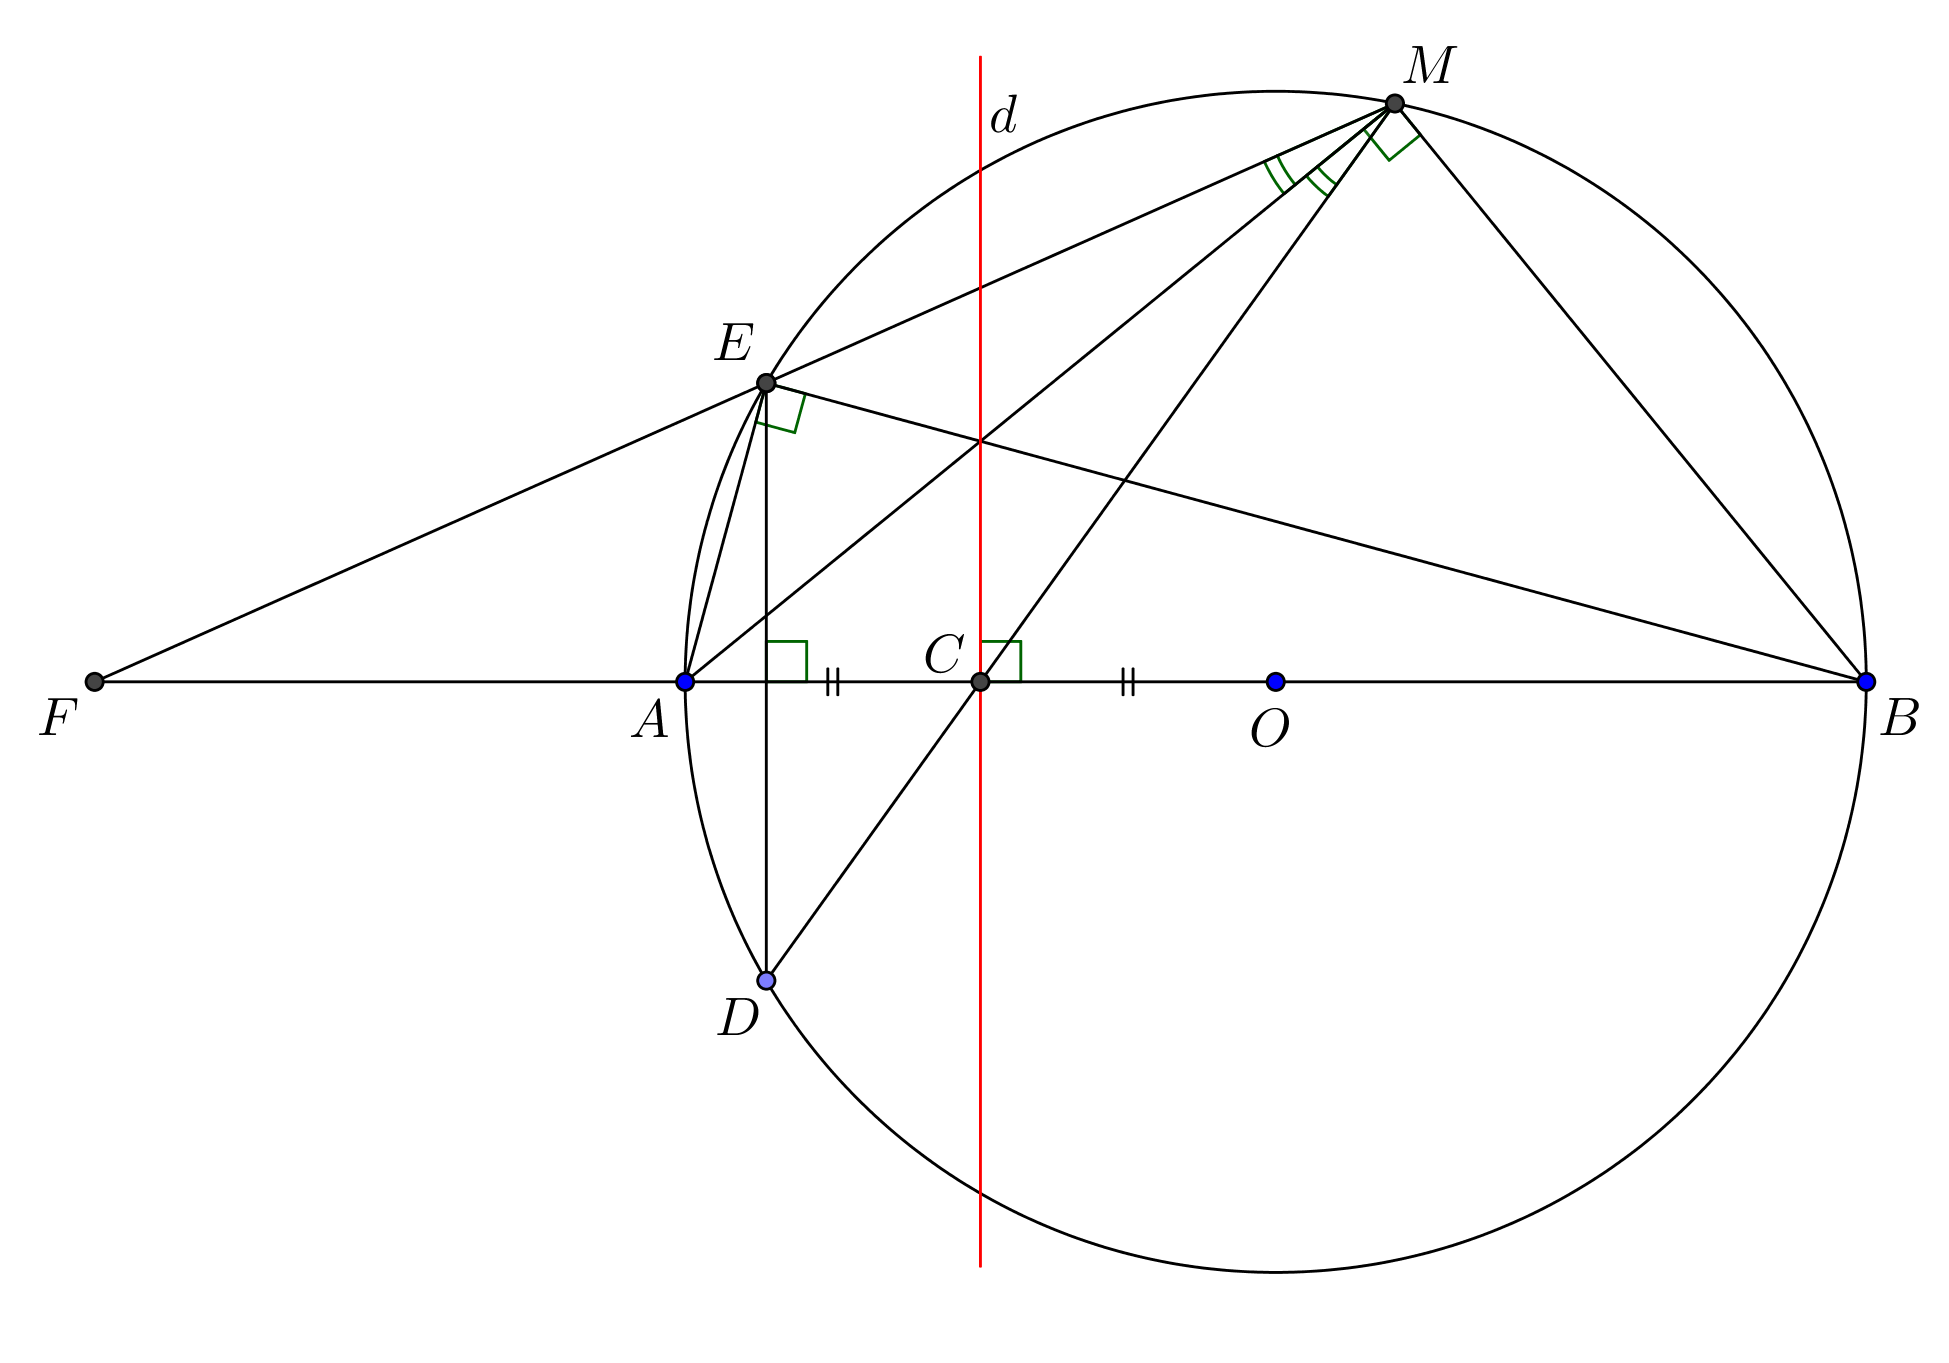
\includegraphics[width= 1\linewidth]{P753-Fig1}
		\caption{\small\textit{\color{thachthuctoanhoc}Hình $1$.}}
		\vspace*{-10pt}
	\end{figure}
	\begin{figure}[H]
		\vspace*{-5pt}
		\centering
		\captionsetup{labelformat= empty, justification=centering}
		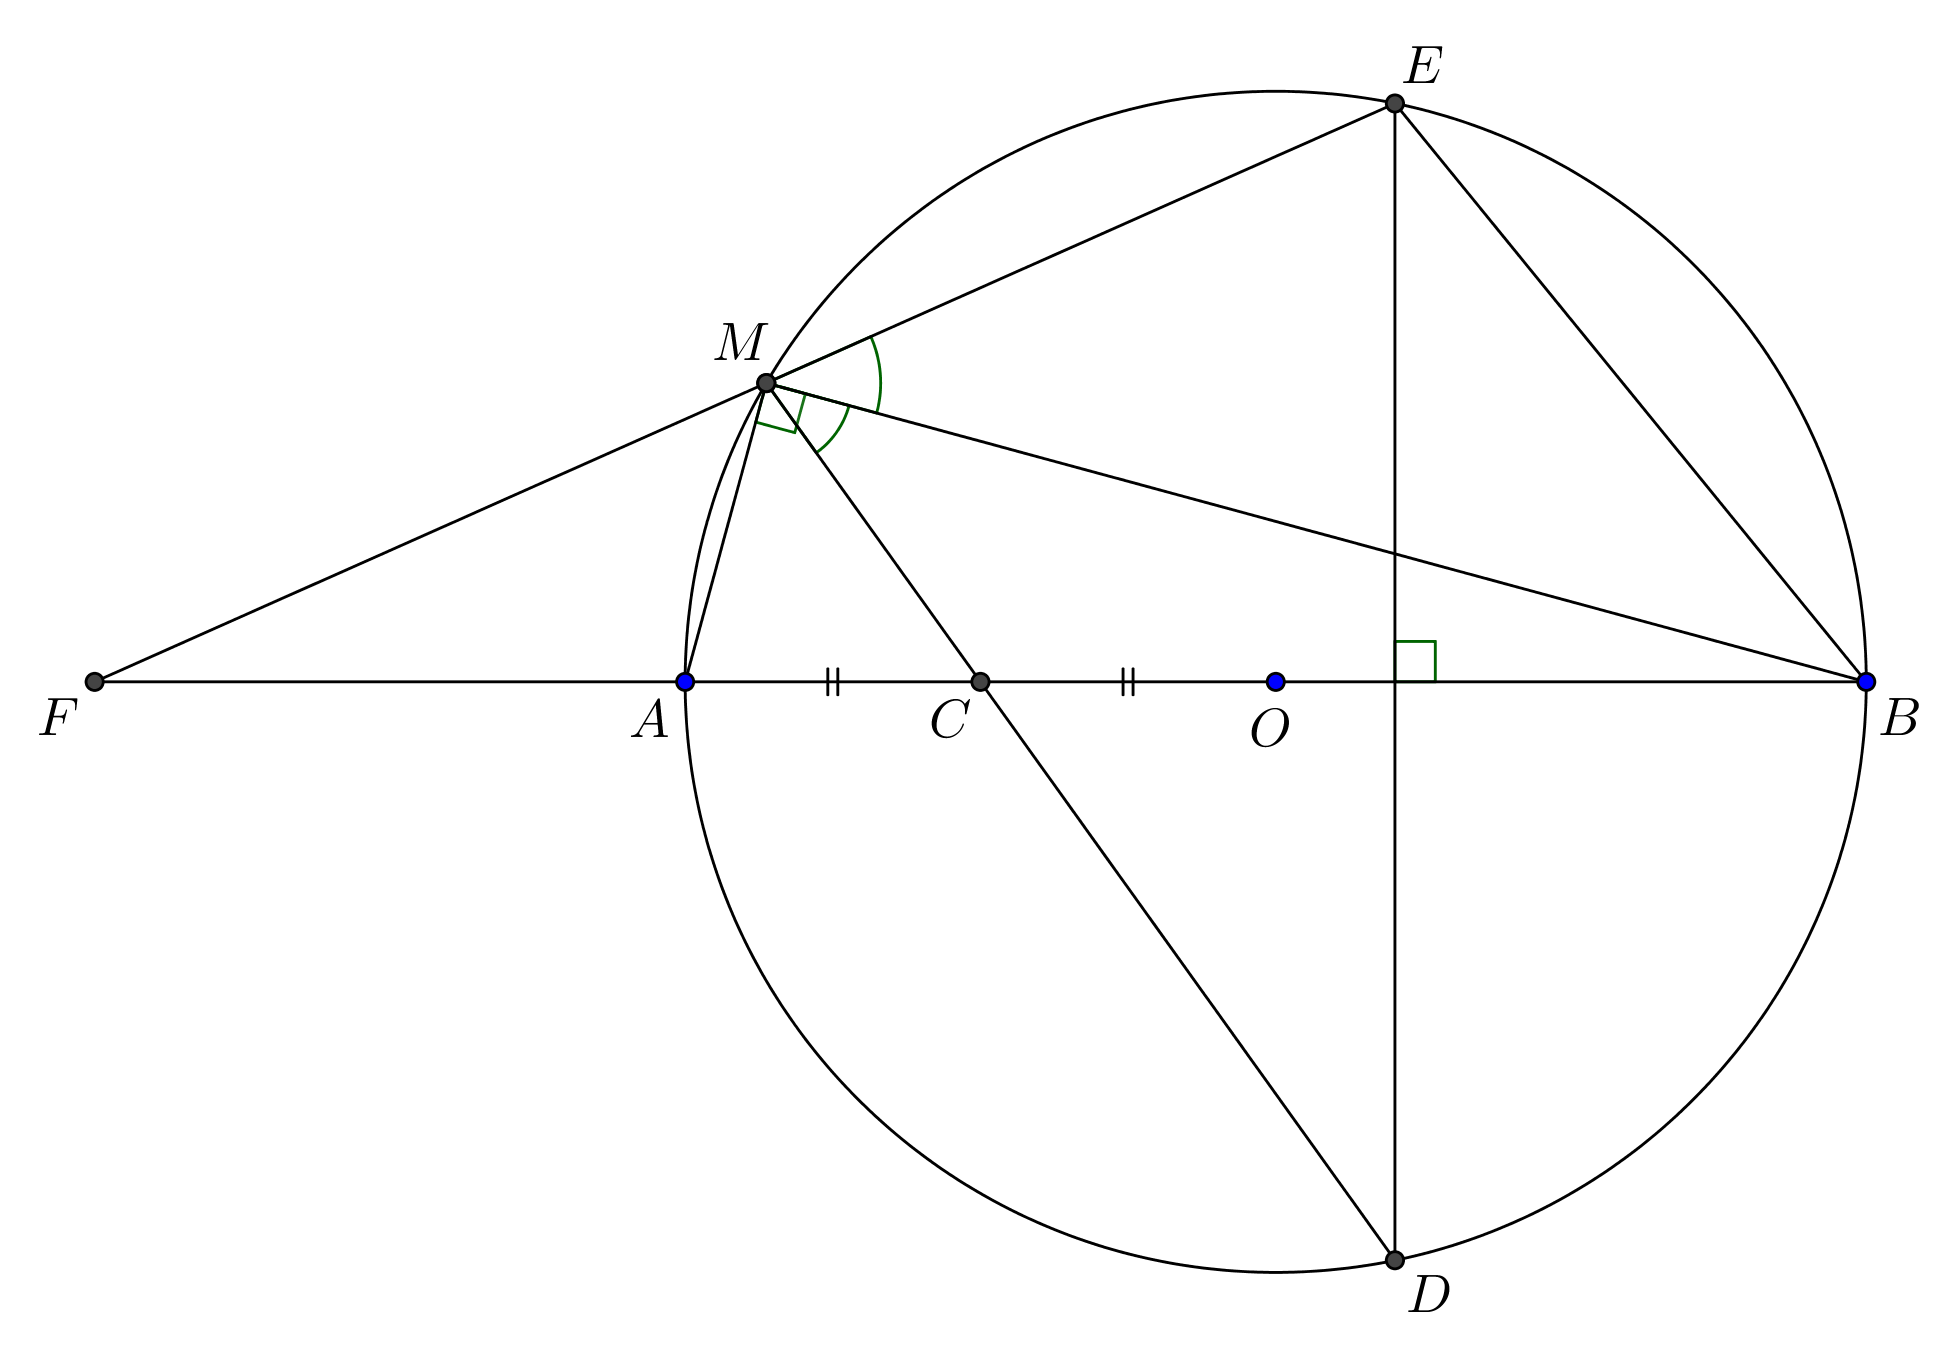
\includegraphics[width= 1\linewidth]{P753-Fig2}
		\caption{\small\textit{\color{thachthuctoanhoc}Hình $2$.}}
		\vspace*{-10pt}
	\end{figure}                                                                    
	Do $AB$ là đường kính của $(O)$ và $DE \bot AB$, nên $D$ và $E$ đối xứng với nhau qua $AB$. Do đó, $A$ và $B$, tương ứng, là điểm chính giữa của cung $EAD$ và của cung $EBD$. \hfill ($1$)
	\vskip 0.05cm
	Lại do $AB$ là đường kính của $(O)$, nên $\angle AMB = 90^\circ$  hay $MA \bot MB.$   \hfill ($2$)
	\vskip 0.05cm
	Từ ($1$) và ($2$) suy ra, $MA$ và $MB$, tương ứng, là phân giác trong và phân giác ngoài của góc $FMC$. Do đó
	\begin{align*}
		\frac{{AC}}{{AF}} = \frac{{BC}}{{BF}} = \frac{{MC}}{{MF}}; \tag{$3$}
	\end{align*}
	suy ra, $\frac{{BF}}{{AF}} = \frac{{BC}}{{AC}}.$ \hfill ($4$)
	\vskip 0.05cm
	Vì $O$ là trung điểm $AB$, $C$ là trung điểm $OA$, và $AB = 2R$, nên
	\begin{align*}
		AC = \frac{R}{2} \text{ và } BC = \frac{3R}{2}. \tag{$5$}
	\end{align*}
	Từ ($4$) và ($5$), suy ra $BF = 3AF$. \hfill ($6$)
	\vskip 0.05cm
	Vì $M, D$ nằm khác phía với $AB$, và $E$ đối xứng với $D$ qua $AB$ (chứng minh trên), nên $M$ và $E$ nằm cùng phía đối với $AB$. Mà $ME$ và $AB$ là hai dây cung không song song của $(O)$, nên đường thẳng $ME$ cắt đường thẳng $AB$ tại điểm $F$, nằm ngoài đoạn thẳng $AB$. Từ đây và ($6$), suy ra, $F$ nằm trên tia đối của tia $AB$, và
	\begin{align*}
		2R = AB = FB - FA = 2FA.
	\end{align*}
	Vì vậy, $FA = R$ và $FB = 3R$. \hfill ($7$)
	\vskip 0.05cm
	Từ ($3$), ($5$), ($7$), suy ra  $MC = \frac{1}{2}MF$ \hfill ($8$)
	\vskip 0.05cm
	Có thể xảy ra hai trường hợp sau, đối với vị trí tương đối giữa $M$ và $O$:
	\vskip 0.05cm
	-- Trường hợp $1$: $M$ nằm cùng phía với $O$, đối với $d$. (Xem Hình $1$.)
	\vskip 0.05cm
	-- Trường hợp $2$: $M$ nằm khác phía với $O$, đối với $d$. (Xem Hình $2$.)
	\vskip 0.05cm
	Vì $F$ nằm trên tia đối của tia $AB$ (chứng minh trên), nên $F$ nằm khác phía với $O$, đối với $d$.
	\vskip 0.05cm
	Từ định nghĩa của $E$, dễ thấy, $E$ và $M$ nằm khác phía nhau, đối với $d$.
	\vskip 0.05cm
	Vì thế, ở trường hợp $1$, $F$ và $E$ cùng nằm khác phía với $M$, đối với $d$; ở trường hợp $2$, $F$ và $M$ cùng nằm khác phía với $E$, đối với $d$.
	\vskip 0.05cm
	Suy ra, ở trường hợp $1$, $E$ nằm giữa $F$ và $M$; ở trường hợp $2$, $M$ nằm giữa $F$ và $E$.
	\vskip 0.05cm
	Do đó:
	\vskip 0.05cm
	-- Với trường hợp $1$, xét hai tam giác $FAE$ và $FMB$, ta có:
	\begin{align*}
		\angle EFA = \angle BFM,\\
		\angle FAE = \angle FMB \text{ (vì cùng bù với $\angle EAB$)}.
	\end{align*}
	Vì thế, $\Delta FAE \sim \Delta FMB$.
	\vskip 0.05cm
	-- Với trường hợp $2$, xét hai tam giác $FAM$ và $FEB$, ta có:
	\begin{align*}
		&\angle MFA = \angle BFE,\\
		&\angle FAM = \angle FEB \text{ (vì cùng bù với $\angle MAB$)}.
	\end{align*}
	Vì thế, $\Delta FAM  \Delta FEB$.
	\vskip 0.05cm
	Do vậy, trong cả hai trường hợp, ta đều có
	\begin{align*}
		\frac{FA}{FE} = \frac{FM}{FB}. \tag{$9$}
	\end{align*}
	Từ ($8$), ($9$), ($7$), suy ra
	\begin{align*}
		EF \cdot MC &= FE \cdot \left( {\frac{1}{2}FM} \right) = \frac{1}{2}\left( {FA \cdot FB} \right) \\
		&= \frac{{3{R^2}}}{2}.
	\end{align*}
	Do đó, theo bất đẳng thức trung bình cộng -- trung bình nhân, ta có:
	\begin{align*}
		EF + MC \ge 2\sqrt {EF \cdot MC}  = \sqrt 6 R;
	\end{align*}
	đẳng thức xảy ra khi và chỉ khi $MC = \frac{{\sqrt 6 R}}{2}.$
	\vskip 0.05cm  
	Dễ thấy, khi $MC = \frac{{\sqrt 6 R}}{2}.$  thì $M$ không trùng $A$, không trùng $B$, và đồng thời, không là giao điểm của $d$ và $(O)$.
	\vskip 0.05cm
	Vì vậy, tổng $EF + MC$ có giá trị nhỏ nhất khi và chỉ khi $M$ là giao điểm của $(O)$ và đường tròn tâm $C$, bán kính $\frac{{\sqrt 6 R}}{2}.$ 
	\vskip 0.05cm
	Ta có điều cần tìm theo yêu cầu đề bài.
	\vskip 0.05cm
	\textbf{\color{thachthuctoanhoc}Bình luận và Nhận xét}
	\vskip 0.05cm
	$\pmb{1.}$ Rất tiếc, tất cả các lời giải Tạp chí đã nhận được từ bạn đọc đều là lời giải chưa đúng, do người giải bài hoặc chưa xét hết các cấu hình có thể, hoặc tuy xét hết nhưng xét sai một trong các cấu hình đó.
	\vskip 0.05cm
	$\pmb{2.}$ Bài toán dưới đây là một bài toán, mà người chấm bài khai thác được từ bài đã ra. Mời các bạn đọc có quan tâm cùng xem xét.
	\vskip 0.05cm
	\textbf{\color{thachthuctoanhoc}Bài toán đề xuất.} Cho đường tròn $(O)$ đường kính $AB$. Gọi $C$ là trung điểm của $OA$. $M$ là một điểm di động trên $(O)$, sao cho $M$ không trùng với $A$, $B$, và giao điểm của $(O)$ với đường thẳng vuông góc với $AB$ tại $C$. Đường thẳng $MC$ cắt $(O)$ tại điểm thứ hai $D$. Gọi $E$ là điểm đối xứng với $D$ qua $AB$. Các đường thẳng $AE$, $BM$ cắt nhau tại $F$; các đường thẳng $AM$, $BE$ cắt nhau tại $G$. Chứng minh rằng, đường thẳng FG đi qua một điểm cố định.
	\begin{flushright}
		\textbf{\color{thachthuctoanhoc}Hạ Vũ Anh}
	\end{flushright}
	{\color{thachthuctoanhoc}{\usefont{T5}{qag}{b}{n} P754.}}
	(Mức $B$) Cho $a, b, c$ là các số thực dương. Chứng minh rằng
	\begin{align*}
		&\frac{b+c}{\sqrt{\!a^2\!+\!b c}\!+\!\!\sqrt{\!a(b+c)}}\!+\!\frac{c\!+\!a}{\sqrt{\!b^2\!+\!c a}\!+\!\!\sqrt{\!b(c\!+\!a)}}\\
		&+\frac{a+b}{\sqrt{c^2+a b}+\sqrt{c(a+b)}} \geq \frac{3}{\sqrt{2}} .
	\end{align*}
	\textbf{\color{thachthuctoanhoc}Lời giải} (\textit{dựa theo đa số lời giải Tạp chí đã nhận được từ bạn đọc})\textbf{\color{thachthuctoanhoc}.}
	\vskip 0.05cm
	Kí hiệu $P$ là biểu thức ở vế trái của bất đẳng thức cần chứng minh theo yêu cầu đề bài.
	\vskip 0.05cm
	Theo bất đẳng thức Cauchy -- Schwarz, ta có:
	\begin{align*}
		&\sqrt {{a^2} + bc}  + \sqrt {a\left( {b + c} \right)}  \\
		\le &\sqrt {\left( {1 + 1} \right)\left( {{a^2} + bc + a\left( {b + c} \right)} \right)} \\
		 = &\sqrt {2\left( {a + b} \right)\left( {a + c} \right)} .
	\end{align*}
	Bằng cách hoàn toàn tương tự, ta thu được các bất đẳng thức sau:
	\begin{align*}
		\sqrt {{b^2} \!+\! ca}  \!+\! \sqrt {b\left( {c \!+\! a} \right)}  \le \sqrt {2\left( {b \!+\! c} \right)\left( {b \!+\! a} \right)} ,\\
		\sqrt {{c^2} \!+\! ab}  \!+\! \sqrt {c\left( {a \!+\! b} \right)}  \le \sqrt {2\left( {c \!+\! a} \right)\left( {c \!+\! b} \right)} .
	\end{align*}
	Từ đó, do $a, b, c > 0$, suy ra
	\begin{align*}
			&P \\
			\ge &\frac{{b + c}}{{\sqrt {2\left( {a + b} \right)\left( {a + c} \right)} }} + \frac{{c + a}}{{\sqrt {2\left( {b + c} \right)\left( {b + a} \right)} }}\\
			& + \frac{{a + b}}{{\sqrt {2\left( {c + a} \right)\left( {c + b} \right)} }}\\
			 \ge &\frac{3}{{\sqrt 2 }} \cdot \sqrt[3]{\frac{{b + c}}{{\sqrt {\left( {a + b} \right)\left( {a + c} \right)} }}}\\
			 &\times\sqrt[3]{\frac{{c + a}}{{\sqrt {\left( {b + c} \right)\left( {b + a} \right)} }}\cdot\frac{{a + b}}{{\sqrt {\left( {c + a} \right)\left( {c + b} \right)} }}}\\
			 = &\frac{3}{{\sqrt 2 }}.
	\end{align*}
	Ta có điều phải chứng minh theo yêu cầu đề bài.
	\vskip 0.05cm
	\textbf{\color{thachthuctoanhoc}Bình luận và Nhận xét}
	\vskip 0.05cm
	$\pmb{1.}$ Từ lời giải trên, dễ thấy, dấu ``=" ở bất đẳng thức của đề bài xảy ra khi và chỉ khi $a = b = c$.
	\vskip 0.05cm
	$\pmb{2.}$ Tất cả các lời giải Tạp chí đã nhận được, từ bạn đọc, đều là lời giải đúng.
	\begin{flushright}
		\textbf{\color{thachthuctoanhoc}Võ Quốc Bá Cẩn}
	\end{flushright}
	{\color{thachthuctoanhoc}{\usefont{T5}{qag}{b}{n} P755.}}
	(Mức $B$) Trong một hình chữ nhật có kích thước $10 \times  5$, lấy $1351$ điểm đôi một phân biệt tùy ý. Chứng minh rằng, tồn tại một hình tròn bán kính bằng   chứa ít nhất $4$ điểm trong số các điểm đã lấy.
	\vskip 0.05cm
	\textbf{\color{thachthuctoanhoc}Lời giải} (\textit{dựa theo đa số lời giải Tạp chí nhận được từ bạn đọc})\textbf{\color{thachthuctoanhoc}.}
	\begin{figure}[H]
		\vspace*{-5pt}
		\centering
		\captionsetup{labelformat= empty, justification=centering}
		\definecolor{wwqqzz}{rgb}{0.4,0.,0.6}
\begin{tikzpicture}[thachthuctoanhoc,scale=0.45]
	\draw  (0.,6.)-- (12.,6.);
	\draw  (12.,6.)-- (12.,0.);
	\draw  (0.,0.)-- (12.,0.);
	\draw  (0.,6.)-- (0.,0.);
	\draw  (1.1338716279069738,6.)-- (1.133871627906975,0.);
	\draw  (0.,1.133871627906975)-- (12.,1.133871627906974);
	\draw  (0.,4.866128372093026)-- (12.,4.866128372093026);
	\draw  (10.866128372093026,6.)-- (10.866128372093026,0.);
	\draw (5.343362935538321,8.270314911314662) node[anchor=north west] {$30$ cột};
	\draw (-3.298792695495564,3.71276020042118) node[anchor=north west] {$15$ hàng};
	\draw (1.9036990027885163,4.099722392855532) node[anchor=north west] {$\ldots \ldots$};
	\draw (7.235178098550715,4.2287097903336495) node[anchor=north west] {$\ldots \ldots$};
	\draw (5.644333529653929,5.217613170999217) node[anchor=north west] {$\vdots$};
	\draw (5.687329328813302,3.1108190121899653) node[anchor=north west] {$\vdots$};
		\draw [fill=white] (0.,0.) circle (1.5pt);
		\draw[color=wwqqzz] (-0.246090955180112,-0.4363344184582641) node {$A$};
		\draw [fill=white] (0.,6.) circle (1.5pt);
		\draw[color=wwqqzz] (-0.4180741518176022,6.614976643678822) node {$B$};
		\draw [fill=white] (12.,0.) circle (1.5pt);
		\draw[color=wwqqzz] (12.308682399356679,0.0796151714542056) node {$D$};
		\draw [fill=white] (12.,6.) circle (1.5pt);
		\draw[color=wwqqzz] (12.308682399356679,6.528985045360077) node {$C$};
\end{tikzpicture}
		\vspace*{-10pt}
	\end{figure}
	Gọi $A, B, C, D$ là bốn đỉnh của hình chữ nhật cho trong đề bài (xem Hình vẽ).
	\vskip 0.05cm
	Kẻ $14$ đoạn thẳng song song, cách đều nhau, và cùng song song với $AD$, $BC$; mỗi đoạn thẳng đều có một đầu mút nằm trên cạnh $AB$, và đầu mút còn lại nằm trên cạnh $CD$.
	\vskip 0.05cm
	Tiếp theo, kẻ $29$ đoạn thẳng song song, cách đều nhau, và cùng song song với $AB$, $DC$; mỗi đoạn thẳng đều có một đầu mút nằm trên cạnh $BC$, và đầu mút còn lại nằm trên cạnh $AD$.
	\vskip 0.05cm
	Các đoạn thẳng kẻ được đã biến hình chữ nhật $ABCD$ thành một bảng ô vuông, gồm $15$ hàng và $30$ cột, mà mỗi hàng, mỗi cột, đều có độ rộng bằng  $\frac{1}{3}$ (vì $AB = 5$, $BC = 10$ (theo giả thiết), và
	\begin{align*}
		5:15 = 10:30 = \frac{1}{3}).
	\end{align*}
	Do đó, $1351$ điểm đã lấy thuộc
	\begin{align*}
		15 \cdot 30 = 450
	\end{align*}
	hình vuông cạnh $\frac{1}{3}$.
	\vskip 0.05cm 
	Theo nguyên lý Dirichlet, trong số các điểm đó, tồn tại ít nhất
	\begin{align*}
		\left[ {\frac{{1351}}{{450}}} \right] + 1 = 4
	\end{align*}
	điểm cùng thuộc một hình vuông, gọi là $H$, trong số các hình vuông ấy.  \hfill ($*$)
	\vskip 0.05cm
	Gọi $r$ là bán kính đường tròn ngoại tiếp hình vuông $H$, ta có:
	\begin{align*}
		r = \frac{1}{2} \cdot \sqrt {{{\left( {\frac{1}{3}} \right)}^2} + {{\left( {\frac{1}{3}} \right)}^2}}  = \frac{{\sqrt 2 }}{6} < \frac{1}{4}.
	\end{align*}
	Vì thế, hình tròn có tâm là tâm của $H$ và có bán kính bằng $\frac{1}{4}$ sẽ phủ kín $H$. Mà $H$ chứa ít nhất bốn điểm trong số các điểm đã lấy (theo ($*$)), nên hình tròn này chứa ít nhất bốn điểm trong số các điểm đã lấy. Ta có điều phải chứng minh theo yêu cầu đề bài.
	\vskip 0.05cm
	\textbf{\color{thachthuctoanhoc}Bình luận và Nhận xét}
	\vskip 0.05cm
	$\pmb{1.}$ Trong số tất cả lời giải tạp chí đã nhận được từ bạn đọc, rất tiếc, có hai lời giải sai, do người giải bài đã \textit{ngộ nhận} rằng, có thể phân chia hình chữ nhật đã cho thành $400$ hình vuông cạnh $\frac{\sqrt{2}}{4}$, hoặc thành $450$ hình vuông cạnh $\frac{1}{9}$.
	\vskip 0.05cm 
	$\pmb{2.}$ Trong số các bạn đọc đã gửi lời giải tới Tạp chí, có một vài bạn sử dụng thuật ngữ chưa đúng, trong các lập luận của mình; chẳng hạn, ``điểm được phủ trong hình" (\textit{diễn đạt đúng phải là}: ``điểm được phủ \textit{bởi} hình"), ....
	\begin{flushright}
		\textbf{\color{thachthuctoanhoc}Nguyễn Khắc Minh}
	\end{flushright}
	{\color{thachthuctoanhoc}{\usefont{T5}{qag}{b}{n} P756.}}
	(Mức $B$) Ta gọi số nguyên dương $n$ là ``số đẹp", nếu trong $22$ số: $5$, $n + 5$, $2n + 5$, $\ldots$, $21n + 5$, tồn tại một số có cùng số dư với tích tất cả các số đó, trong phép chia cho $23$. Hãy tìm tất cả các số đẹp.
	\vskip 0.05cm
	\textbf{\color{thachthuctoanhoc}Lời giải} (\textit{dựa theo ý giải của các bạn: Đỗ Viết Hoàng Long, lớp $11$A, trường THPT chuyên Quang Trung, tỉnh Bình Phước; và Đỗ Duy Quang, lớp $12$T$1$, trường THPT chuyên Nguyễn Quang Diêu, tỉnh Đồng Tháp})\textbf{\color{thachthuctoanhoc}.}
	\vskip 0.05cm
	Với mỗi số nguyên dương $n$, ký hiệu $T_n$ là tích tất cả các số $5$, $n + 5$, $2n + 5$, $\ldots$, $21n + 5$.
	\vskip 0.05cm
	Khi đó, theo đề bài, $n$ là số đẹp, nếu trong $22$ số $kn + 5$, $k = 0, 1, 2, \ldots, 21$, có ít nhất một số có cùng số dư với  $T_n$, trong phép chia cho $23$.
	\vskip 0.05cm
	Xét các trường hợp sau:
	\vskip 0.05cm
	$\bullet$ \textit{Trường hợp} $1$: $n \equiv 0\left( {\bmod 23} \right).$
	\vskip 0.05cm  
	Khi đó,
	\begin{align*}
		kn + 5 \equiv 5\left( {\bmod 23} \right)\forall k = \overline {0,21} . \tag{$1$}
	\end{align*}
	Vì vậy, ${T_n} \equiv {5^{22}}\left( {\bmod 23} \right).$ \hfill ($2$)
	\vskip 0.05cm
	Do $23$ là số nguyên tố, và $(5, 23) = 1$, nên
	\begin{align*}
		{5^{22}} \equiv 1\left( {\bmod 23} \right)	\text{(theo Định lý Fermat nhỏ).} \tag{$3$}
	\end{align*}
	Từ ($2$) và ($3$), suy ra  ${T_n} \equiv 1\left( {\bmod 23} \right).$ \hfill ($4$)
	\vskip 0.05cm
	Vì $5 \ne 1$, nên ($1$) và ($4$) cho thấy số $n$ trong trường hợp này \textit{không} là số đẹp.
	\vskip 0.05cm
	$\bullet$ \textit{Trường hợp} $2$:
	\vskip 0.05cm  
	Khi đó, do $23$ là số nguyên tố, nên $(n, 23) = 1$.
	\vskip 0.05cm
	Vì vậy, với $i, j \in \{0; 1; 2; \ldots; 21\}$ và $i \ne j$, ta có:
	\begin{align*}
		&in + 5 \equiv jn + 5\left( {\bmod 23} \right)\\
		\Leftrightarrow &\left( {i - j} \right)n \equiv 0\left( {\bmod 23} \right)\\
		\Leftrightarrow & i \equiv j\left( {\bmod 23} \right) \Leftrightarrow i = j.
	\end{align*}
	Do đó, tập hợp $S$ các số dư trong phép chia lần lượt $22$ số $5$, $n + 5$, $2n + 5$, $\ldots$, $21n + 5$ cho $23$ sẽ là tập hợp gồm $22$ số tự nhiên đôi một khác nhau, trong phạm vi từ $0$ đến $22$. \hfill  ($5$)
	\vskip 0.05cm
	-- Nếu $n$ là số sao cho $0 \in S$ thì hiển nhiên $n$ là số đẹp, vì khi đó, ${T_n} \equiv 0\left( {\bmod 23} \right).$
	\vskip 0.05cm  
	-- Xét $n$ là số sao cho $0 \notin S$.
	\vskip 0.05cm  
	Khi đó, theo ($5$), $S$ là tập hợp gồm $22$ số nguyên dương đầu tiên. Vì thế, với lưu ý $23$ là số nguyên tố, theo định lý Wilson, ta có:
	\begin{align*}
		{T_n} \equiv 22! \equiv  - 1 \equiv 22\left( {\bmod 23} \right). \tag{$6$}
	\end{align*}
	Vì $22 \in S$ nên ($6$) cho thấy $n$ là một số đẹp.
	\vskip 0.05cm
	Vậy, tóm lại, tất cả các số đẹp là tất cả các số nguyên dương không chia hết cho $23$.
	\vskip 0.05cm
	\textbf{\color{thachthuctoanhoc}Bình luận và Nhận xét}
	\vskip 0.05cm
	$\pmb{1.}$ Định lý Wilson được nhắc tới trong Lời giải trên là kết quả sau:
	\vskip 0.05cm
	\textbf{\color{thachthuctoanhoc}Định lý Wilson.} \textit{Nếu $p$ là số nguyên tố thì}
	\begin{align*}
		\left( {p - 1} \right)! \equiv  - 1\left( {\bmod p} \right).
	\end{align*}
	$\pmb{2.}$ Nếu chưa biết định lý Wilson, bạn đọc có thể chứng minh ($6$) bằng cách tính cụ thể $22!$.
	\vskip 0.05cm
	$\pmb{3.}$ Tất cả lời giải Tạp chí đã nhận được từ bạn đọc đều là lời giải đúng.
	\begin{flushright}
		\textbf{\color{thachthuctoanhoc}Lưu Thị Thanh Hà}
	\end{flushright}
	{\color{thachthuctoanhoc}{\usefont{T5}{qag}{b}{n} P757.}}
	(Mức $A$) Với mỗi số nguyên dương $n$, ký hiệu  $a_n$ là nghiệm thực lớn nhất của phương trình
	\begin{align*}
		{x^{2023}} - n{x^{2022}} - n{x^{2021}} -  \cdots  - nx + 1 = 0.
	\end{align*}
	Xác định tất cả các số thực $C$, để
	\begin{align*}
		{a_1} + {a_2} +  \cdots  + {a_n} > C \cdot {n^2}
	\end{align*}
	với mọi số nguyên dương $n$.
	\vskip 0.05cm
	\textbf{\color{thachthuctoanhoc}Lời giải} (\textit{dựa theo Đáp án của BBT Tạp chí})\textbf{\color{thachthuctoanhoc}.}
	\vskip 0.05cm
	Xét số nguyên dương $n$ tùy ý.
	\vskip 0.05cm
	Với mỗi số nguyên dương $k > 1$, đặt
	\begin{align*}
		{P_k}\left( x \right) = {x^k} - n{x^{k - 1}} - n{x^{k - 2}} -  \cdots  - nx + 1.
	\end{align*}
	Khi đó, phương trình đã nêu trong đề bài được viết thành
	\begin{align*}
		{P_{2023}}\left( x \right) = 0. \tag{$1$}
	\end{align*}
	Với $x \ge n + 1$, ta có:
	\begin{align*}
			&{P_k}\left( x \right) \\
			= &{x^{k - 1}}\left( {x - n} \right) - n{x^{k - 2}} -  \cdots  - nx + 1\\
			 \\
			\ge &{x^{k - 1}} - n{x^{k - 2}} -  \cdots  - nx + 1 = {P_{k - 1}}\left( x \right),
	\end{align*}
	với mọi số nguyên dương $k > 2$.
	\vskip 0.05cm
	Do đó, với $x \ge n + 1$, ta có:
	\begin{align*}
		{P_{2023}}\!\!\left( x \right) &\!\ge\! {P_{2022}}\!\!\left( x \right) \!\ge\! {P_{2021}}\!\!\left( x \right) \!\ge\!  \cdots  \!\ge\! {P_2}\!\!\left( x \right)\\
		& = {x^2} - nx + 1 = x\left( {x - n} \right) + 1\\
		&\ge x + 1 > 0.
	\end{align*}
	Lại có:
	\begin{align*}
		&{P_{2023}}\left( n \right) \\
		= \,\,&{n^{2023}} - {n^{2023}} - {n^{2022}} -  \cdots  - {n^2} + 1 < 0.
	\end{align*}
	Vì thế, phương trình ($1$) có nghiệm trong khoảng $(n, n + 1)$ và vô nghiệm trong $[n+ 1, + \infty)$.
	\vskip 0.05cm 
	Do đó, vì là nghiệm thực lớn nhất của phương trình ($1$), nên $a_n \in (n, n+1)$.
	\vskip 0.05cm  
	Từ đây, do tính tùy ý của $n$, ta có
	\begin{align*}
		{a_n} \in \left( {n,n + 1} \right)\forall n \in \mathbb{N^*}. \tag{$2$}
	\end{align*}
	Với mỗi $n \in \mathbb{N^*}$,  đặt
	\begin{align*}
		{s_n} = \frac{{{a_1} + {a_2} +  \cdots  + {a_n}}}{{{n^2}}}.
	\end{align*}
	Theo bài ra, ta cần tìm tất cả các số thực $C$, sao cho
	\begin{align*}
		{s_n} > C\forall n \in  \mathbb{N^*}. \tag{$3$}
	\end{align*}
	Từ ($2$), suy ra
	\begin{align*}
		\frac{1}{{{n^2}}} \cdot \sum\limits_{i = 1}^n i  < {s_n} < \frac{1}{{{n^2}}} \cdot \sum\limits_{i = 1}^n {\left( {i + 1} \right)} \forall n \in \mathbb{N^*}. \tag{$4$}
	\end{align*}
	Ta có:
	\begin{align*}
		&(4) \\
		\Leftrightarrow\, &\frac{{n\left( {n + 1} \right)}}{{2{n^2}}} < {s_n}\\
		& < \frac{1}{{{n^2}}}\left( {\frac{{\left( {n + 1} \right)\left( {n + 2} \right)}}{2} - 1} \right)\forall n \in \mathbb{N^*}\\
		\Leftrightarrow \,&\frac{1}{2} + \frac{1}{{2n}} < {s_n} < \frac{1}{2} + \frac{3}{{2n}}\forall n \in \mathbb{N^*}. \tag{$5$}
	\end{align*}
	Dễ thấy, ${\left( {\frac{1}{2} + \frac{1}{{2n}}} \right)_{n \ge 1}},$ ${\left( {\frac{1}{2} + \frac{3}{{2n}}} \right)_{n \ge 1}}$ là các dãy hội tụ, và
	\begin{align*}
		\mathop {\lim }\limits_{n \to  + \infty } \left( {\frac{1}{2} + \frac{1}{{2n}}} \right) = \mathop {\lim }\limits_{n \to  + \infty } \left( {\frac{1}{2} + \frac{3}{{2n}}} \right) = \frac{1}{2}.
	\end{align*}
	Vì vậy, từ ($5$), theo định lys kẹp, suy ra ${\left( {{s_n}} \right)_{n \ge 1}}$  là dãy hội tụ, và
	\begin{align*}
		\mathop {\lim }\limits_{n \to  + \infty } {s_n} = \frac{1}{2}. \tag{$6$}
	\end{align*}
	$\bullet$ Giả sử $C$ là một số thực thỏa mãn ($3$).
	\vskip 0.05cm
	Khi đó, do ($6$) nên $C \le \frac{1}{2}$.
	\vskip 0.05cm  
	$\bullet$ Ngược lại, giả sử $C$ là một số thực không vượt quá  $\frac{1}{2}$.
	\vskip 0.05cm
	Khi đó, theo ($5$), ta có:
	\begin{align*}
		{s_n} > \frac{1}{2} + \frac{1}{{2n}} > \frac{1}{2} \ge C\forall n \in \mathbb{N^*}.
	\end{align*}
	Do đó, $C$ là số thực thỏa mãn ($3$).
	\vskip 0.05cm
	$\bullet$ Vậy, tất cả các số thực $C$ thỏa mãn yêu cầu đề bài là: $C \le \frac{1}{2}$.
	\vskip 0.05cm 
	\textbf{\color{thachthuctoanhoc}Bình luận và Nhận xét}
	\vskip 0.05cm
	Cho tới thời điểm bản thảo vào Nhà in, Tạp chí mới chỉ nhận được đúng một lời giải từ bạn đọc. Rất tiếc, lời giải này là một lời giải không đạt yêu cầu, do có một số khẳng định mang tính cốt yếu được nêu ra một cách cảm tính, không có bất cứ lí giải hay chứng minh nào.
	\begin{flushright}
		\textbf{\color{thachthuctoanhoc}Nguyễn Khắc Minh}
	\end{flushright}
	{\color{thachthuctoanhoc}{\usefont{T5}{qag}{b}{n} P758.}}
	(Mức $A$) Tìm số thực $k$ lớn nhất, sao cho
	\begin{align*}
		a + b + c - 3 \ge k\left( {a - b} \right)\left( {b - c} \right)\left( {c - a} \right)
	\end{align*}
	với mọi số thực không âm $a, b, c$, thỏa mãn
	\begin{align*}
		ab + bc + ca = 3.
	\end{align*}
	\textbf{\color{thachthuctoanhoc}Lời giải} (\textit{của người chấm bài})\textbf{\color{thachthuctoanhoc}.}
	\vskip 0.05cm
	Trong phần trình bày dưới đây, $\mathbb{R^+}$  ký hiệu tập các số thực không âm.
	\vskip 0.05cm
	Giả sử $k$ là số thực thỏa mãn yêu cầu đề bài; nghĩa là, với mọi $a,b,c \in \mathbb{R^+}$  thỏa mãn
	\begin{align*}
		ab + bc + ca = 3, \tag{$1$}
	\end{align*}
	đều có 
	\begin{align*}
		a \!+\! b \!+\! c \!-\! 3 \!\ge\! k\left( {a \!-\! b} \right)\left( {b \!-\! c} \right)\left( {c \!-\! a} \right). \tag{$2$}
	\end{align*}
	Bằng kiểm tra trực tiếp, ta thấy, các giá trị $a = 1$, $b = 3$, $c = 0$ là các số thực không âm, thỏa mãn ($1$). Vì vậy, theo ($2$), ta có:
	\begin{align*}
		1 + 3 + 0 - 3 \ge k\left( {1 - 3} \right)\left( {3 - 0} \right)\left( {0 - 1} \right);
	\end{align*}
	suy ra, $k \le \frac{1}{6}$. \hfill ($3$)
	\vskip 0.05cm
	Tiếp theo, ta sẽ chứng minh $k = \frac{1}{6}$  thỏa mãn yêu cầu đề bài; nghĩa là, ta sẽ chứng minh
	\begin{align*}
		a + b + c - 3 \ge \frac{1}{6}\left( {a - b} \right)\left( {b - c} \right)\left( {c - a} \right),
	\end{align*}
	với mọi $a,b,c \in \mathbb{R^+}$  thỏa mãn ($1$).
	\vskip 0.05cm
	Thật vậy, do $a,b,c \in \mathbb{R^+}$  thỏa mãn ($1$), nên $a + b + c > 0$. Vì thế, với lưu ý tới ($1$), ta có:
	\begin{align*}
		&(4) \\
		\Leftrightarrow \,&{\left( {a + b + c} \right)^2} - 9 \\
		&\ge \frac{{\left( {b - a} \right)\left( {b - c} \right)\left( {a - c} \right)\left( {a + b + c + 3} \right)}}{6}\\
		\Leftrightarrow \,&{\left( {a + b + c} \right)^2} - 3\left( {ab + bc + ca} \right) \\
		&\ge \frac{{\left( {b - a} \right)\left( {b - c} \right)\left( {a - c} \right)}}{{2\left( {ab + bc + ca} \right)}}\\
		&\quad\times \frac{\left( {a + b + c + \sqrt {3\left( {ab + bc + ca} \right)} } \right)}{{2\left( {ab + bc + ca} \right)}}\\
		\Leftrightarrow \,&{\left( {b - a} \right)^2} + {\left( {b - c} \right)^2} + {\left( {a - c} \right)^2} \\
		&\ge \frac{{\left( {b - a} \right)\left( {b - c} \right)\left( {a - c} \right)}}{{ab + bc + ca}}.\\
		&\quad\times \frac{\left( {a + b + c + \sqrt {3\left( {ab + bc + ca} \right)} } \right)}{{ab + bc + ca}}.
	\end{align*}
	Do tính đối xứng vòng quanh, nên không mất tính tổng quát, giả sử $c = \min\{a, b, c\}$.
	\vskip 0.05cm
	-- Nếu $a \ge b$, hoặc $a = c$, thì ($5$) hiển nhiên là một bất đẳng thức đúng.
	\vskip 0.05cm
	-- Xét $b > a > c \ge 0$.
	\vskip 0.05cm
	Đặt $x = b - c$ và $y = a - c$; ta có $x > y > 0$, và do đó
	\begin{align*}
			&\frac{{a + b + c}}{{ab + bc + ca}} \\
			=& \frac{{{{\left( {a + b} \right)}^2} + ac + bc}}{{\left( {a + b} \right)\left( {ab + bc + ca} \right)}}\\
			 =& \frac{{{a^2} + ab + {b^2}}}{{\left( {a + b} \right)\left( {ab + bc + ca} \right)}} + \frac{1}{{a + b}}\\
			 \le& \frac{{{a^2} + ab + {b^2}}}{{\left( {a + b} \right)ab}} + \frac{1}{{a + b}} = \frac{1}{a} + \frac{1}{b}\\
			\le& \frac{1}{{a - c}} + \frac{1}{{b - c}} = \frac{1}{x} + \frac{1}{y}, \tag{$6$}
	\end{align*}
	\begin{align*}
		&\frac{{\sqrt {3\left( {ab + bc + ca} \right)} }}{{ab + bc + ca}} = \sqrt {\frac{3}{{ab + bc + ca}}}  \\
		\le &\sqrt {\frac{3}{{ab}}}  \le \sqrt {\frac{3}{{\left( {a - c} \right)\left( {b - c} \right)}}}  = \sqrt {\frac{3}{{xy}}} . \tag{$7$}
	\end{align*}
	Kí hiệu $P$, $Q$, tương ứng, là biểu thức ở vế phải và biểu thức ở vế trái của ($5$).
	\vskip 0.05cm
	Do ($6$) và ($7$), với lưu ý $b - a = x - y$, ta có:
	\begin{align*}
			P \le& xy\left( {x - y} \right)\left( {\frac{1}{x} + \frac{1}{y} + \sqrt {\frac{3}{{xy}}} } \right)\\
			 = \,&\left( {x - y} \right)\left( {x + y + \sqrt {3xy} } \right) \\
			 = \,&{x^2} - {y^2} + \frac{{\left( {2\sqrt {xy} } \right)\left( {\sqrt 3 \left( {x - y} \right)} \right)}}{2}\\
			 \le\,& {x^2} - {y^2} + \frac{{4xy + 3{{\left( {x - y} \right)}^2}}}{4} \\
			= \,&\frac{{7{x^2} - 2xy - {y^2}}}{4} \\
			= \,&{x^2} + {y^2} + {\left( {x - y} \right)^2} - \frac{{{{\left( {x - 3y} \right)}^2}}}{4}\\
			 \le\,& {x^2} + {y^2} + {\left( {x - y} \right)^2} = Q.
	\end{align*}
	Bất đẳng thức ($5$) được chứng minh, và vì thế, ($4$) được chứng minh. Từ đây và ($3$) suy ra, số thực $k$ lớn nhất thỏa mãn yêu cầu đề bài là  $k = \frac{1}{6}$.
	\vskip 0.05cm
	\textbf{\color{thachthuctoanhoc}Bình luận và Nhận xét}
	\vskip 0.05cm
	$\pmb{1.}$ Chứng minh bất đẳng thức ($4$) với ràng buộc ($1$) (theo ký hiệu ở Lời giải trên) là một bài toán khó. Vì thế, bài đã ra là một bài toán rất khó.
	\vskip 0.05cm
	$\pmb{2.}$ Tất cả các lời giải người chấm bài đã nhận được từ Ban biên tập Tạp chí đều là lời giải đúng; tuy nhiên, phần chứng minh bất đẳng thức ($4$) có quá nhiều các tính toán cồng kềnh, với độ phức tạp rất cao. Có cảm giác, người giải bài đã phải thực hiện các tính toán đó với sự trợ giúp của các phần mềm tính toán.
	\begin{flushright}
		\textbf{\color{thachthuctoanhoc}Võ Quốc Bá Cẩn}
	\end{flushright}
	{\color{thachthuctoanhoc}{\usefont{T5}{qag}{b}{n} P759.}}
	(Mức $A$) Cho tam giác $ABC$ nội tiếp đường tròn $(O)$, có các đường cao $BE$, $CF$ cắt nhau tại $H$. Gọi $M$, $N$ tương ứng là trung điểm của $AH$, $EF$. Gọi $P$ là điểm đối xứng với $N$ qua $BC$. Chứng minh rằng, $\angle BMP = \angle NMC$.
	\vskip 0.05cm 
	\textbf{\color{thachthuctoanhoc}Lời giải} (\textit{của người chấm bài})\textbf{\color{thachthuctoanhoc}.}
	\vskip 0.05cm
	Theo phát biểu của đề bài, ta hiểu $E$ và $F$ là hai điểm không trùng nhau. Vì thế, ta hiểu, tam giác $ABC$ cho trong đề bài \textit{không} vuông tại $A$. Phần trình bày dưới đây là lời giải cho bài ra với giả thiết đó.
	\vskip 0.05cm
	Xét hai trường hợp sau:
	\vskip 0.05cm
	$\bullet$ \textit{Trường hợp $1$: Tam giác $ABC$ cân tại $A$.}
	\vskip 0.05cm
	Trong trường hợp này, $AH$ là đường trung trực của $BC$, và tất cả các điểm $M, N, P$ đều thuộc $AH$ (xem Hình $1$). Vì thế, kết luận của bài ra hiển nhiên đúng.
	\begin{figure}[H]
		\vspace*{-10pt}
		\centering
		\captionsetup{labelformat= empty, justification=centering}
		\definecolor{qqwuqq}{rgb}{0.,0.39215686274509803,0.}
		\definecolor{uuuuuu}{rgb}{0.26666666666666666,0.26666666666666666,0.26666666666666666}
		\definecolor{xdxdff}{rgb}{0.49019607843137253,0.49019607843137253,1.}
		\definecolor{qqqqff}{rgb}{0.,0.,1.}
		\begin{tikzpicture}[thachthuctoanhoc,scale=0.6]
			\draw [shift={(2.,2.75)},pattern color=qqwuqq,fill=qqwuqq,fill opacity=0.10000000149011612] (0,0) -- (-128.6598082540901:0.6) arc (-128.6598082540901:-90.:0.6) -- cycle;
			\draw [shift={(2.,2.75)},pattern color=qqwuqq,fill=qqwuqq,fill opacity=0.10000000149011612] (0,0) -- (-90.:0.8) arc (-90.:-51.3401917459099:0.8) -- cycle;
			\draw[pattern color=qqwuqq,fill=qqwuqq,fill opacity=0.10000000149011612] (0.07350889359326482,1.1470177871865295) -- (0.3264911064067352,1.0205266807797944) -- (0.4529822128134704,1.2735088935932648) -- (0.2,1.4) -- cycle; 
			\draw[pattern color=qqwuqq,fill=qqwuqq,fill opacity=0.10000000149011612] (3.5470177871865296,1.2735088935932646) -- (3.6735088935932647,1.0205266807797944) -- (3.926491106406735,1.1470177871865295) -- (3.8,1.4) -- cycle; 
			\draw  (-1.,-1.)-- (5.,-1.);
			\draw  (2.,5.)-- (-1.,-1.);
			\draw  (2.,5.)-- (5.,-1.);
			\draw  (0.2,1.4)-- (3.8,1.4);
			\draw  (-1.,-1.)-- (2.,2.75);
			\draw  (2.,2.75)-- (5.,-1.);
			\draw  (2.,5.)-- (2.,-3.4);
			\draw  (0.2,1.4)-- (5.,-1.);
			\draw (1.8,5.78) node[anchor=north west] {$A$};
			\draw (-1.5,-0.76) node[anchor=north west] {$B$};
			\draw (5.,-0.76) node[anchor=north west] {$C$};
			\draw (3.86,2.14) node[anchor=north west] {$E$};
			\draw (-0.36,2.06) node[anchor=north west] {$F$};
			\draw (1.56,1.32) node[anchor=north west] {$H$};
			\draw (1.46,3.44) node[anchor=north west] {$M$};
			\draw (2.06,2.1) node[anchor=north west] {$N$};
			\draw (1.78,-3.22) node[anchor=north west] {$P$};
			\draw  (-1.,-1.)-- (3.8,1.4);
			\draw [fill=white] (-1.,-1.) circle (1.5pt);
			\draw [fill=white] (5.,-1.) circle (1.5pt);
			\draw [fill=white] (2.,5.) circle (1.5pt);
			\draw [fill=white] (2.,0.5) circle (1.5pt);
			\draw [fill=white] (0.2,1.4) circle (1.5pt);
			\draw [fill=white] (3.8,1.4) circle (1.5pt);
			\draw [fill=white] (2.,1.4) circle (1.5pt);
			\draw [fill=white] (2.,2.75) circle (1.5pt);
			\draw [fill=white] (2.,-3.4) circle (1.5pt);
		\end{tikzpicture}
		\caption{\small\textit{\color{thachthuctoanhoc}Hình $1$.}}
		\vspace*{-10pt}
	\end{figure}
	$\bullet$ \textit{Trường hợp $2$: Tam giác $ABC$ không cân tại $A$.}
	\vskip 0.05cm
	Giả sử $AB < AC$; trường hợp $AB > AC$ được xét tương tự.
	\vskip 0.05cm
	Xảy ra hai trường hợp nhỏ sau:
	\vskip 0.05cm
	$\diamondsuit$ \textit{Trường hợp $2.1$: $AH \parallel EF$}. (Xem Hình $2$.)
	\begin{figure}[H]
		\vspace*{-5pt}
		\centering
		\captionsetup{labelformat= empty, justification=centering}
		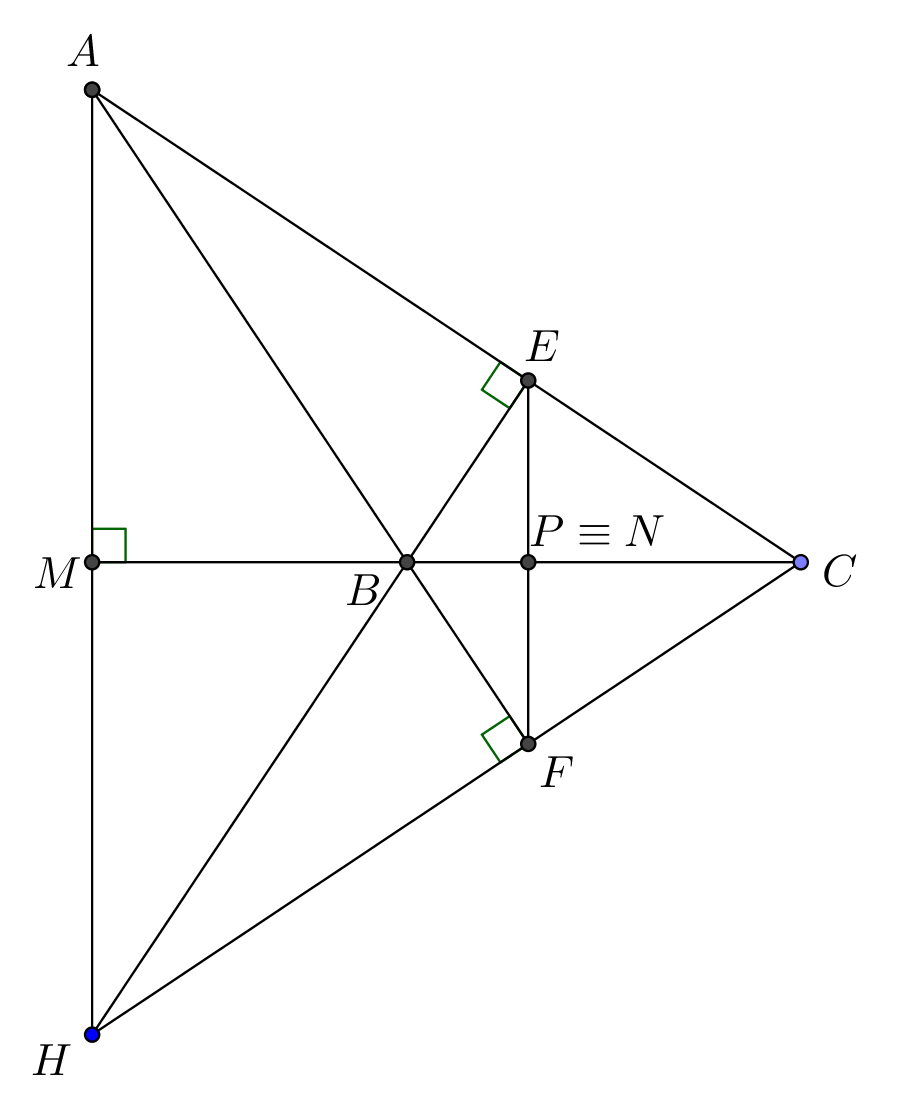
\includegraphics[scale =0.5]{P759-Fig2}
		\caption{\small\textit{\color{thachthuctoanhoc}Hình $2$.}}
		\vspace*{-10pt}
	\end{figure}
	Trong trường hợp này, các điểm $M$ và $N$ cùng thuộc $BC$; do đó, $P \equiv N$. Vì thế
	\begin{align*}
		\angle BMP = \angle NMC = {0^\circ}
	\end{align*}
	Kết luận của đề bài được chứng minh.
	\vskip 0.05cm
	$\diamondsuit$ \textit{Trường hợp $2.2$: $AH$ không song song $EF$.} (Xem Hình $3$.)
	\begin{figure}[H]
		\vspace*{-5pt}
		\centering
		\captionsetup{labelformat= empty, justification=centering}
		\definecolor{qqwuqq}{rgb}{0.,0.39215686274509803,0.}
		\definecolor{uuuuuu}{rgb}{0.26666666666666666,0.26666666666666666,0.26666666666666666}
		\definecolor{qqqqff}{rgb}{0.,0.,1.}
		\begin{tikzpicture}[thachthuctoanhoc,scale=0.65]
			\draw[pattern color=qqwuqq,fill=qqwuqq,fill opacity=0.10000000149011612] (3.7228427124746184,-2.) -- (3.7228427124746184,-1.7171572875253809) -- (3.44,-1.7171572875253809) -- (3.44,-2.) -- cycle; 
			\draw[pattern color=qqwuqq,fill=qqwuqq,fill opacity=0.10000000149011612] (6.041810368997817,1.7986068797457995) -- (6.235513361301193,1.5925021714717806) -- (6.441618069575211,1.7862051637751564) -- (6.247915077271836,1.9923098720491752) -- cycle; 
			\draw[pattern color=qqwuqq,fill=qqwuqq,fill opacity=0.10000000149011612] (2.2694417228224633,-0.693956093541116) -- (2.546450932873403,-0.7511041254140893) -- (2.6035989647463764,-0.4740949153631495) -- (2.3265897546954366,-0.4169468834901762) -- cycle; 
			\draw[pattern color=qqwuqq,fill=qqwuqq,fill opacity=0.10000000149011612] (4.570095128458256,-2.) -- (4.570095128458256,-1.7171572875253813) -- (4.2872524159836365,-1.7171572875253813) -- (4.2872524159836365,-2.) -- cycle; 
			\draw  (3.44,4.98)-- (2.,-2.);
			\draw  (10.,-2.)-- (3.44,4.98);
			\draw  (3.44,2.166676217765043)-- (6.,-2.);
			\draw  (3.44,2.166676217765043)-- (10.,-2.);
			\draw  (3.44,2.166676217765043)-- (4.2872524159836365,-4.7876814942795);
			\draw  (6.247915077271836,1.9923098720491752)-- (-0.25,-2.);
			\draw  (-0.25,-2.)-- (10.,-2.);
			\draw  (2.3265897546954366,-0.4169468834901762)-- (10.,-2.);
			\draw  (2.,-2.)-- (6.247915077271836,1.9923098720491752);
			\draw  (3.44,-2.)-- (3.44,4.98);
			\draw  (2.,-2.)-- (3.44,2.166676217765043);
			\draw (3.24,5.78) node[anchor=north west] {$A$};
			\draw (1.64,-1.78) node[anchor=north west] {$B$};
			\draw (10.,-1.76) node[anchor=north west] {$C$};
			\draw (6.22,2.7) node[anchor=north west] {$E$};
			\draw (1.98,0.22) node[anchor=north west] {$F$};
			\draw (2.9,2.74) node[anchor=north west] {$M$};
			\draw (4.14,1.58) node[anchor=north west] {$N$};
			\draw (4.04,-4.58) node[anchor=north west] {$P$};
			\draw (6.,-1.76) node[anchor=north west] {$I$};
			\draw (-0.76,-1.72) node[anchor=north west] {$S$};
			\draw (2.96,0.92) node[anchor=north west] {$Q$};
			\draw (3.14,-1.76) node[anchor=north west] {$D$};
			\draw (3.34,-0.44) node[anchor=north west] {$H$};
			\draw  (2.,-2.)-- (4.2872524159836365,-4.7876814942795);
			\draw  (4.2872524159836365,-4.7876814942795)-- (10.,-2.);
			\draw  (2.,-2.)-- (3.44,0.26713080313855947);
			\draw  (4.2872524159836365,0.7876814942794995)-- (10.,-2.);
			\draw  (4.2872524159836365,-2.)-- (4.2872524159836365,0.7876814942794995);
			\draw  (4.1972524159836375,-0.6411592528602502) -- (4.377252415983637,-0.6411592528602502);
			\draw  (4.1972524159836375,-0.5711592528602503) -- (4.377252415983637,-0.5711592528602503);
			\draw  (4.2872524159836365,-2.)-- (4.2872524159836365,-4.7876814942795);
			\draw  (4.377252415983637,-3.35884074713975) -- (4.1972524159836375,-3.35884074713975);
			\draw  (4.377252415983637,-3.42884074713975) -- (4.1972524159836375,-3.42884074713975);
			\draw  (6.,-1.0502272926867584) circle (4.11121249700829cm);
				\draw [fill=white] (3.44,4.98) circle (1.5pt);
				\draw [fill=white] (2.,-2.) circle (1.5pt);
				\draw [fill=white] (10.,-2.) circle (1.5pt);
				\draw [fill=white] (2.3265897546954366,-0.4169468834901762) circle (1.5pt);
				\draw [fill=white] (3.44,-0.6466475644699142) circle (1.5pt);
				\draw [fill=white] (6.247915077271836,1.9923098720491752) circle (1.5pt);
				\draw [fill=white] (-0.25,-2.) circle (1.5pt);
				\draw [fill=white] (4.2872524159836365,0.7876814942794995) circle (1.5pt);
				\draw [fill=white] (3.44,2.166676217765043) circle (1.5pt);
				\draw [fill=white] (6.,-2.) circle (1.5pt);
				\draw [fill=white] (3.44,-2.) circle (1.5pt);
				\draw [fill=white] (4.2872524159836365,-4.7876814942795) circle (1.5pt);
				\draw [fill=white] (3.44,0.26713080313855947) circle (1.5pt);
				\draw [fill=white] (4.2872524159836365,-2.) circle (1.5pt);
		\end{tikzpicture}
		\caption{\small\textit{\color{thachthuctoanhoc}Hình $3$.}}
		\vspace*{-10pt}
	\end{figure}
	Gọi $I$ là trung điểm của $BC$; gọi $S$, $Q$ lần lượt là giao điểm của các đường thẳng $BC$, $AH$ với đường thẳng $EF$.
	\vskip 0.05cm
	Theo tính chất của tứ giác toàn phần, ta có $M, N, I$ thẳng hàng, và
	\begin{align*}
		\left( {SQ,EF} \right) =  - 1.
	\end{align*}
	Từ đó, do $N$ là trung điểm của $EF$, nên 
	\begin{align*}
		\overline {SQ}  \cdot \overline {SN}  = \overline {SE}  \cdot \overline {SF} . \tag{$1$}
	\end{align*}
	Từ định nghĩa các điểm $E, F$ suy ra, bốn điểm $B, C, E, F$ cùng thuộc đường tròn đường kính $BC$. Do đó
	\begin{align*}
		\overline {SB}  \cdot \overline {SC}  = \overline {SE}  \cdot \overline {SF} . \tag{$2$}
	\end{align*}
	Từ ($1$) và ($2$) suy ra, bốn điểm $B, C, N, Q$ cùng thuộc một đường tròn. \hfill ($3$)                                             
	\vskip 0.05cm
	Từ định nghĩa điểm $H$, ta có $HE \bot EA$ và $HF \bot FA$. Do đó, bốn điểm $A, H, E, F$ cùng thuộc đường tròn tâm $M$, đường kính $AH$. Vì thế, theo định lý Brokard, $M$ là trực tâm tam giác $BCQ$; và do đó, $Q$ là trực tâm tam giác $BCM$. Từ đây và ($3$), do tính đối xứng, ta được:
	\begin{align*}
		\left( {MC;MB} \right) &\equiv \left( {QB;QC} \right) \equiv \left( {NB;NC} \right) \\
		&\equiv \left( {PC;PB} \right)\left( {\bmod \pi } \right).
	\end{align*}
	Do đó, bốn điểm $B, C, M, P$ cùng thuộc một đường tròn.    \hfill ($4$)
	\vskip 0.05cm
	Dễ thấy, $\Delta BHA \sim \Delta BFE$; mà $M$, $N$ tương ứng là trung điểm của $HA$, $FE$, nên $\Delta BMA \sim \Delta BNE$. Suy ra
	\begin{align*}
		\frac{{BN}}{{BM}} = \frac{{BE}}{{BA}}. \tag{$5$}
	\end{align*}
	Một cách tương tự, ta cũng chứng minh được
	\begin{align*}
		\frac{{CN}}{{CM}} = \frac{{CF}}{{CA}}. \tag{$6$}
	\end{align*}
	Lại có $\Delta ABE \sim \Delta ACF$ (dễ thấy), nên
	\begin{align*}
		\frac{{BE}}{{BA}} = \frac{{CF}}{{CA}}. \tag{$7$}
	\end{align*}
	Do $N$ và $P$ đối xứng với nhau qua $BC$, nên $CP = CN$ và $BP = BN$ \hfill  ($8$)
	\vskip 0.05cm
	Từ ($5$), ($6$), ($7$), ($8$), suy ra
	\begin{align*}
		\frac{{CP}}{{CM}} = \frac{{BP}}{{BM}}. \tag{$9$}
	\end{align*}
	Từ ($4$) và ($9$) suy ra, $BMCP$ là một tứ giác điều hòa. Mà $MI$ là đường trung tuyến và $MP$ là đường đối trung của tam giác $MBC$, nên
	\begin{align*}
		\angle BMP = \angle IMC = \angle NMC.
	\end{align*}
	Ta có điều phải chứng minh theo yêu cầu đề bài.
	\vskip 0.05cm
	\textbf{\color{thachthuctoanhoc}Bình luận và Nhận xét}
	\vskip 0.05cm
	$\pmb{1.}$ Lời giải trên cho thấy, giả thiết tam giác $ABC$ nội tiếp đường tròn $(O)$ là một giả thiết không cần thiết.
	\vskip 0.05cm
	$\pmb{2.}$ Rất tiếc, tất cả các bạn đã gửi lời giải đến Tạp chí đều chỉ giải bài đã ra trong trường hợp tam giác $ABC$ không cân tại $A$, và đồng thời $AH$ không song song $EF$.
	\begin{flushright}
		\textbf{\color{thachthuctoanhoc}Hạ Vũ Anh}
	\end{flushright}
	{\color{thachthuctoanhoc}{\usefont{T5}{qag}{b}{n} P760.}}
	(Mức $A$) Cho dãy số  $(x_n)$ xác định bởi $x_1 = 4$  và
	\begin{align*}
		{x_{n + 1}} = 45{x_n} + \sqrt {2024x_n^2 + 16} 
	\end{align*}
	với mọi số nguyên dương $n$.
	\vskip 0.05cm
	Tìm tất cả các số nguyên $a$, sao cho ${a^n}\left( {\frac{{{x_{2n}}}}{{{x_n}}} + 2} \right)$  là số chính phương, với mọi số nguyên dương $n$.
	\vskip 0.05cm
	\textbf{\color{thachthuctoanhoc}Lời giải} (\textit{dựa theo Đáp án của BBT Tạp chí})\textbf{\color{thachthuctoanhoc}.}
	\vskip 0.05cm
	Từ hệ thức xác định dãy $(x_n)$  suy ra dãy đó là dãy tăng thực sự, $x_2 = 360$  và
	\begin{align*}
		x_n^2 - 90{x_{n + 1}}{x_n} + x_{n + 1}^2 - 16 = 0, \tag{$1$}
	\end{align*}
	với mọi $n \ge 1$.
	\vskip 0.05cm
	Trong ($1$), thay $n$ bởi $n + 1$, ta được:
	\begin{align*}
		x_{n + 2}^2 - 90{x_{n + 1}}{x_{n + 2}} + x_{n + 1}^2 - 16 = 0, \tag{$2$}
	\end{align*}
	với mọi $n \ge 1$.
	\vskip 0.05cm
	Vì $(x_n)$  là dãy tăng thực sự (chứng minh trên), nên ${x_n} \ne {x_{n + 2}},$ với mọi $n \ge 1$. Do đó, từ ($1$) và ($2$) suy ra, với mọi $n \ge 1$, $x_n$  và $x_{n+2}$  là hai nghiệm của phương trình (ẩn $x$) sau:
	\begin{align*}
		{x^2} - 90{x_{n + 1}}x + x_{n + 1}^2 - 16 = 0.
	\end{align*}
	Vì thế, theo định lý Vi--et, ta có:
	\begin{align*}
		{x_{n + 2}} = 90{x_{n + 1}} - {x_n}, \tag{$3$}
	\end{align*}
	với mọi $n \ge 1$.
	\vskip 0.05cm
	Từ $x_1 = 4$, $x_2 = 360$ và ($3$), theo công thức xác định số hạng tổng quát của dãy số được cho bởi hệ thức truy hồi tuyến tính cấp $2$, ta được:
	\begin{align*}
		{x_n} = \frac{{{{\left( {45 + 2\sqrt {506} } \right)}^n} - {{\left( {45 - 2\sqrt {506} } \right)}^n}}}{{\sqrt {506} }},
	\end{align*}
	với mọi $n \ge 1$.
	\vskip 0.05cm
	Suy ra, $x_n > 0$  và
	\begin{align*}
		\frac{{{x_{2n}}}}{{{x_n}}} = {\left( {45 + 2\sqrt {506} } \right)^n} + {\left( {45 - 2\sqrt {506} } \right)^n},
	\end{align*}
	với mọi $n \ge 1$.
	\vskip 0.05cm
	Nhận thấy
	\begin{align*}
		&{23^n}\left( {\frac{{{x_{2n}}}}{{{x_n}}} + 2} \right) \\
		= &{\left( {{{\left( {23 + \sqrt {506} } \right)}^n} + {{\left( {23 - \sqrt {506} } \right)}^n}} \right)^2},
	\end{align*}
	với mọi $n \ge 1$.
	\vskip 0.05cm
	Với mỗi $n \in \mathbb{N^*}$  đặt
	\begin{align*}
		{y_n} = {\left( {23 + \sqrt {506} } \right)^n} + {\left( {23 - \sqrt {506} } \right)^n}.
	\end{align*}
	Dễ thấy, ta có  $y_1 = 46$, $y_2 = 2070$, và
	\begin{align*}
		{y_{n + 2}} = 46{y_{n + 1}} - 23{y_n}\forall n \ge 1.
	\end{align*}
	Suy ra, $y_n \in \mathbb{Z}$ với mọi $n \ge 1$. Do đó, ${23^n}\left( {\frac{{{x_{2n}}}}{{{x_n}}} + 2} \right)$  là một số chính phương, với mọi $n \ge 1$. \hfill  ($4$)
	\vskip 0.05cm
	Vì thế, với $a$ là số nguyên tùy ý thỏa mãn yêu cầu đề bài, do với mọi $n \ge 1$,
	\begin{align*}
		\frac{{{a^n}}}{{{{23}^n}}} = \frac{{{a^n}\left( {\frac{{{x_{2n}}}}{{{x_n}}} + 2} \right)}}{{{{23}^n}\left( {\frac{{{x_{2n}}}}{{{x_n}}} + 2} \right)}} \text{ (vì $x_n >0 \,\,\,\forall n \ge 1$)}	
	\end{align*}
	nên $\frac{{{a^n}}}{{{{23}^n}}}$  là bình phương của một số hữu tỷ, với mọi $n \ge 1$.
	\vskip 0.05cm
	Suy ra, $\frac{a}{23}$  là bình phương của một số hữu tỷ. Do đó, $a \in \mathbb{N}$  và tồn tại  $q,p \in \mathbb{N},p \ne 0$ và $(q, p) = 1$, sao cho
	\begin{align*}
		\frac{a}{{23}} = \frac{{{q^2}}}{{{p^2}}}, \text{ hay } ap^2 = 23q^2. \tag{$5$}
	\end{align*}
	Suy ra, $a = 0$, hoặc $a$ là số nguyên dương lớn hơn $1$, mà số mũ của số nguyên tố $23$ trong phân tích chuẩn của $a$ là một số lẻ. Do đó, $a = 0$, hoặc $a$ là một số nguyên dương chia hết cho $23$. Vì vậy, $a$ là số tự nhiên có dạng $a = 23m$, với $m$ là số tự nhiên. Từ đây và ($5$), suy ra
	\begin{align*}
		m{p^2} = {q^2}.
	\end{align*}
	Từ đó, do $(q, p) = 1$, dễ dàng suy ra $p = 1$, và vì thế, $m = q^2$.
	\vskip 0.05cm  
	Như vậy, nếu số nguyên $a$ thỏa mãn yêu cầu đề bài thì $a$ có dạng $a = 23q^2, q \in \mathbb{N}$.
	\vskip 0.05cm   
	Ngược lại, với $a = 23q^2, q\in \mathbb{N}$    ta có:
	\begin{align*}
		{a^n}\left( {\frac{{{x_{2n}}}}{{{x_n}}} + 2} \right) = {23^n}\left( {\frac{{{x_{2n}}}}{{{x_n}}} + 2} \right) \cdot {q^2},
	\end{align*}
	với mọi $n \ge 1$.
	\vskip 0.05cm
	Mà $q^2$ là số chính phương và  ${23^n}\left( {\frac{{{x_{2n}}}}{{{x_n}}} + 2} \right)$ là số chính phương với mọi $n \ge 1$ (theo ($4$)), nên  ${a^n}\left( {\frac{{{x_{2n}}}}{{{x_n}}} + 2} \right)$ là số chính phương với mọi $n \ge 1$.
	\vskip 0.05cm
	Vậy, tất cả các số tự nhiên có dạng $23q^2, q \in \mathbb{N}$  là tất cả các số $a$ thỏa mãn yêu cầu đề bài.
	\vskip 0.05cm
	\textbf{\color{thachthuctoanhoc}Bình luận và Nhận xét}
	\vskip 0.05cm
	Rất tiếc, đến thời điểm bản thảo vào Nhà in, Tạp chí vẫn chưa nhận được lời giải nào từ bạn đọc.
	\begin{flushright}
		\textbf{\color{thachthuctoanhoc}Lưu Thị Thanh Hà}
	\end{flushright}
\end{multicols}
\begin{center}
	\textbf{\color{thachthuctoanhoc}DANH SÁCH HỌC SINH CÓ LỜI GIẢI ĐÚNG}
\end{center}
\begin{multicols}{2}
	\textit{Trong các ngoặc đơn ở phần dưới đây, sau tên lớp là mã hiệu của các bài toán mà học sinh có lời giải đúng.}
	\vskip 0.05cm
	\textbf{\color{thachthuctoanhoc}KHỐI THCS}
	\vskip 0.05cm
	$\bullet$  Trường \textbf{\color{thachthuctoanhoc}THCS Nguyễn Thái Bình}, Tp. Cà Mau, tỉnh Cà Mau: \textit{Lê Nguyễn Hoàng Nhật Đình} (lớp $9$C; P$751$, P$754$, P$755$).
	\vskip 0.05cm
	$\bullet$  Trường \textbf{\color{thachthuctoanhoc}TH\&THCS Archimedes Đông Anh}, Tp. Hà Nội: \textit{Ngô Minh Chấn} (lớp $9$A$3$; P$754$, P$755$).
	\vskip 0.05cm
	$\bullet$  Trường \textbf{\color{thachthuctoanhoc}THCS Lê Quý Đôn}, Quận $3$, Tp. Hồ Chí Minh: \textit{Nguyễn Chánh Thiện} (lớp $9/12$; P$751$, P$752$, P$754$).
	\vskip 0.05cm
	$\bullet$  Trường \textbf{\color{thachthuctoanhoc}THCS Mỹ Hưng}, Tp. Nam Định, tỉnh Nam Định: \textit{Trần Tiến Dũng} (lớp $9$A$1$; P$754$).
	\vskip 0.05cm
	$\bullet$  Trường \textbf{\color{thachthuctoanhoc}THCS Hồ Xuân Hương}, huyện Quỳnh Lưu, tỉnh Nghệ An: \textit{Phạm Quang Thắng} (lớp $7$C; P$754$, P$755$).
	\vskip 0.05cm
	$\bullet$  Trường \textbf{\color{thachthuctoanhoc}THCS Lý Tự Trọng}, Tp. Tam Kỳ, tỉnh Quảng Nam: \textit{Phan Minh Huy} (lớp $9/3$; P$752$, P$754$).
	\vskip 0.05cm
	\textbf{\color{thachthuctoanhoc}KHỐI THPT}
	\vskip 0.05cm
	$\bullet$  Trường \textbf{\color{thachthuctoanhoc}THPT chuyên Quang Trung}, tỉnh Bình Phước: \textit{Đỗ Viết Hoàng Long} (lớp $11$A; P$756$).
	\vskip 0.05cm
	$\bullet$  Trường \textbf{\color{thachthuctoanhoc}THPT chuyên Nguyễn Quang Diêu}, tỉnh Đồng Tháp: \textit{Phạm Tiến Đạt} (lớp $10$T$1$; P$754$, P$755$), \textit{Liêu Vĩ Hào} (lớp $10$T$1$; P$751$, P$754$), \textit{Huỳnh Phúc Vĩnh Nguyên} (lớp $10$T$1$; P$754$), \textit{Đỗ Duy Quang} (lớp $12$T$1$; P$751$, P$752$, P$754$, P$755$, P$756$), \textit{Trần Thị Phương Thảo} (lớp $10$T$1$; P$751$, P$755$), \textit{Võ Hải Yến} (lớp $11$H; P$751$, P$754$).
	\vskip 0.05cm
	$\bullet$  Trường \textbf{\color{thachthuctoanhoc}THPT chuyên Lương Văn Chánh}, tỉnh Phú Yên: \textit{Nguyễn Tấn Nguyên Chương} (lớp $11$ Toán $1$; P$754$), \textit{Huỳnh Trần Gia Huy} (lớp $10$ Toán $1$; P$758$), \textit{Đặng Kỳ Nam} (lớp $10$ Toán $1$; P$751$, P$754$).
	\vskip 0.05cm
	$\bullet$  Trường \textbf{\color{thachthuctoanhoc}THPT chuyên Lê Thánh Tông}, tỉnh Quảng Nam: \textit{Nguyễn Hữu Hoàng Nhật} (lớp $11/1$; P$754$).
	\vskip 0.05cm
	$\bullet$  Trường \textbf{\color{thachthuctoanhoc}THPT chuyên Tiền Giang}, tỉnh Tiền Giang: \textit{Nguyễn Nhật Minh} (lớp $10$ Toán $1$; P$751$).
\end{multicols}

